
\input{"C:/Users/spileggi/Google Drive/STAT 330/Lectures/SlideStyle.tex"}


\title[Lecture 16]{PROC REPORT}
\author[Pileggi]{Shannon Pileggi}

\institute[STAT 330]{STAT 330}

\date{}


\begin{document}

\begin{frame}
\titlepage
\end{frame}

\begin{frame}
\frametitle{OUTLINE\qquad\qquad\qquad} \tableofcontents[hideallsubsections]
\end{frame}


%===========================================================================================================================
\section[Overview]{Overview}
%===========================================================================================================================
\subsection{}
\begin{frame}
\ft{Overview}
\hspace*{-0.3in}
\begin{tabular}{|l|ccc|ccccc|}
\hline
\ttt{PROC}    & Detail  & Summary & Control & N        & sum    & mean & std & \% \\
\hline
\hline
\ttt{PRINT}   &  \gc    &    \rx  & \gc &  \gc    &    \gc  & \rx & \rx      &  \rx   \\
\ttt{MEANS}   &  \rx    &    \gc  & \rx &  \gc    &    \gc  & \gc & \gc      &  \rx    \\
\ttt{FREQ}    &  \rx    &    \gc  & \rx &  \gc    &    \rx  & \rx & \rx      &  \gc \\
\hline
\ttt{REPORT}  &  \gc    &    \gc  & \gc &  \gc    &    \gc  & \gc & \gc      &  \gc \\
\ttt{TABULATE}&  \rx    &    \gc  & \gc &  \gc    &    \gc  & \gc & \gc      &  \gc \\
\ttt{SQL}     &  \gc    &    \gc  & \rx &  \gc    &    \gc  & \gc & \gc      &  \gc  \\
\hline
\end{tabular}
\begin{itemize}
\item Detail: display a row for each observation
\item Summary: display a row for a group of observations
\item Control: many layout/format/display options in output
\item \ttt{SQL}: can additionally combine and sort data
\end{itemize}
\end{frame}

\begin{frame}
\ft{Patents data}
\bi
\item number of utility patent (``patents for inventions'') grants from 2011, by county
\item demographic variables from the American Community Survey
\bi
\item some variables may be missing for smaller counties
\ei
\item San Jose, CA (Santa Clara County)
\bi
\item $3^{rd}$ largest city in CA, $10^{th}$ largest city in US
\item leads all US cities in generating patents
\ei
\ei
\oyo Explore the \ttt{patents} data in SAS.
\end{frame}

\begin{frame}[fragile]
\ft{Syntax}
\bmp{.50\textwidth}
\begin{code}{.}
PROC REPORT DATA = \emph{dataset} ;
   COLUMN \emph{item1} \emph{item2} ...  ;
   DEFINE \emph{item1} / \emph{options} ;
   DEFINE \emph{item2} / \emph{options} ;
RUN;
\end{code}
\emp
\bmp{0.05\textwidth} \hspace{0.05in} \emp
\bmp{0.50\textwidth}
Default properties:
\begin{itemize}
\item Permanent formats/labels automatically applied
\item Character vars left justified, numeric vars right-justified
\end{itemize}
\emp
\vskip10pt
\bi
\item an \emph{item} can be a \emph{variable} or a \emph{statistic}
\item \ttt{COLUMN} specifies \emph{items} to use and their order of appearance
\item \ttt{DEFINE} specifies the \emph{item's} use and display
\ei
\end{frame}

\begin{frame}
\ft{DEFINE usages}
\begin{center}
\fbox{\ttt{DEFINE \emph{var1} / \emph{usage}};}
\end{center}
\vskip10pt
\begin{tabular}{lccl}
\hline
 Usage            & Detail    & Summary & Description \\
\hline
\hline
\ttt{DISPLAY}      &  \gc      &  \rx       & creates 1 row per obs            \\
\ttt{ORDER}        &  \gc      &  \rx       & creates 1 row per obs, ordered          \\
\hline
\ttt{ANALYSIS}     &  \gc      &  \gc       & calculates statistics            \\
\ttt{COMPUTED}     &  \gc      &  \gc       & creates new variable            \\
\hline
\ttt{GROUP}        &  \rx      &  \gc       & values placed in rows            \\
\ttt{ACROSS}       &  \rx      &  \gc       & values placed in columns            \\
\hline
\end{tabular}
\end{frame}

%===========================================================================================================================
\section[Detail Report]{Detail Report}
%===========================================================================================================================
\subsection{}
\begin{frame}
\tableofcontents[currentsection, hideallsubsections]
\end{frame}


\begin{frame}[fragile]
\ft{Getting started}
\hspace{-0.3in}
\bmp{.55\textwidth}
\begin{code}{.}
PROC REPORT DATA = patents ;
RUN ;


PROC REPORT DATA = patents ;
   COLUMN state county patents ;
RUN ;


PROC REPORT DATA = patents ;
   COLUMN state county patents ;
   DEFINE state / \textcolor{OrangeRed}{DISPLAY} ;
   DEFINE county / \textcolor{OrangeRed}{DISPLAY} ;
   DEFINE patents / \textcolor{OrangeRed}{ANALYSIS} ;
RUN ;
\end{code}
\emp
%\bmp{.03\textwidth} \hspace{0.05in} \emp
\bmp{.50\textwidth}
\begin{itemize}
\item[]
\item with no statements, prints all data
\item[]
\item \ttt{COLUMN} specifies variables to print (and order of display)
\item[]
\item equivalent output to previous \ttt{PROC}
\item Default usages:
\item[] \ttt{DISPLAY} for character vars
\item[] \ttt{ANALYSIS} for numeric vars
\end{itemize}
\emp
\end{frame}



\begin{frame}[fragile]
\ft{Getting started - example output}
\hspace{-0.3in}
\bmp{.55\textwidth}
\begin{code}{.}
PROC REPORT DATA = patents ;
   COLUMN state county patents ;
   DEFINE state / \textcolor{OrangeRed}{DISPLAY} ;
   DEFINE county / \textcolor{OrangeRed}{DISPLAY} ;
   DEFINE patents / \textcolor{OrangeRed}{ANALYSIS} ;
RUN ;
\end{code}
\emp
\blankcolumn
\bmp{.50\textwidth}
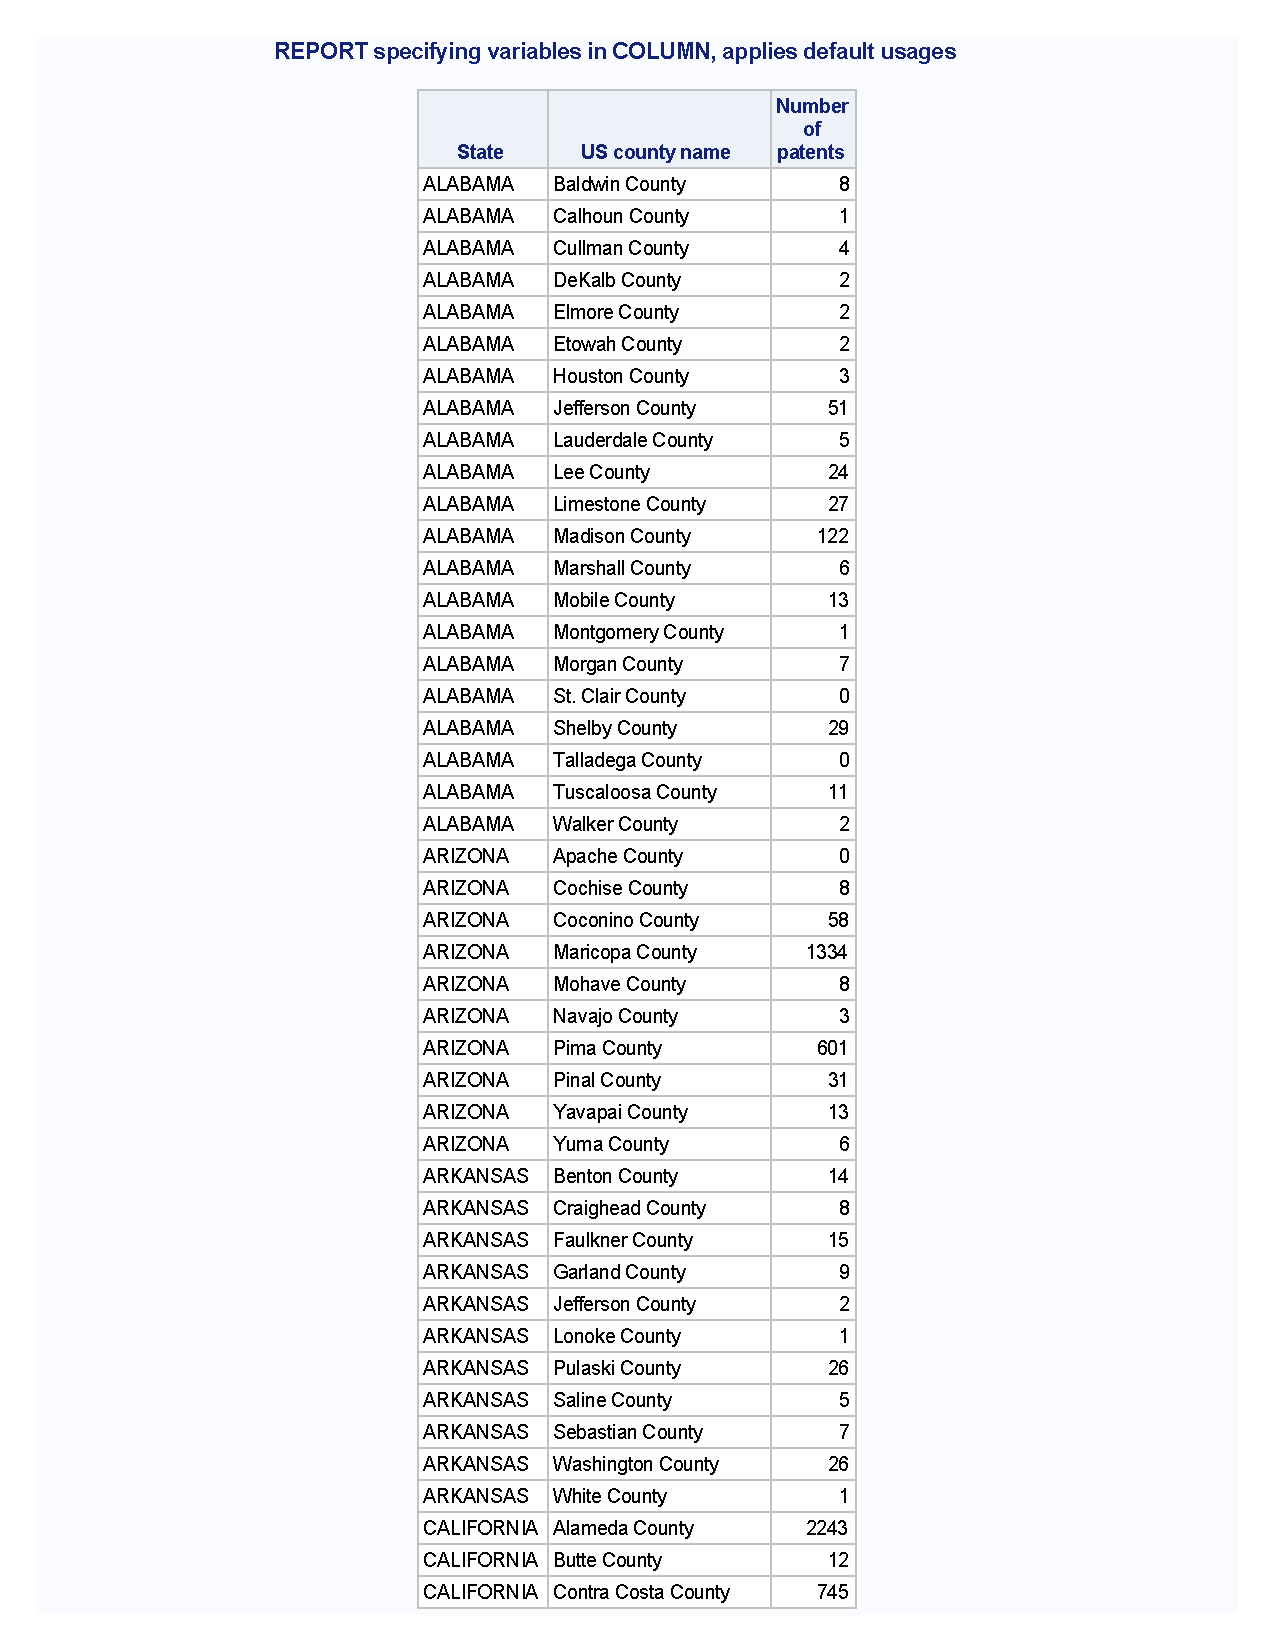
\includegraphics[trim={6.5cm 18cm 6.5cm 1.5cm},clip,width=1.0\textwidth]{L16_basic_detail.pdf}
\emp
\end{frame}

\begin{frame}[fragile]
\ft{ORDER usage and SPANROWS}
\hspace*{-0.3in}
\bmp{.61\textwidth}
\begin{code}{.}
PROC REPORT DATA = patents \textcolor{OrangeRed}{SPANROWS};
   COLUMN state county patents ;
   DEFINE state / \textcolor{OrangeRed}{ORDER} ;
   DEFINE county / \textcolor{OrangeRed}{ORDER} ;
   DEFINE patents / \textcolor{OrangeRed}{ANALYSIS} ;
RUN ;
\end{code}
\begin{itemize}
\item With \ttt{ORDER}:
\bi
\item rows arranged by ascending values
\item repetitious printing is suppressed
\ei
\item \ttt{SPANROWS} merges cells with same values
\end{itemize}
\emp
\blankcolumn
\bmp{.50\textwidth}
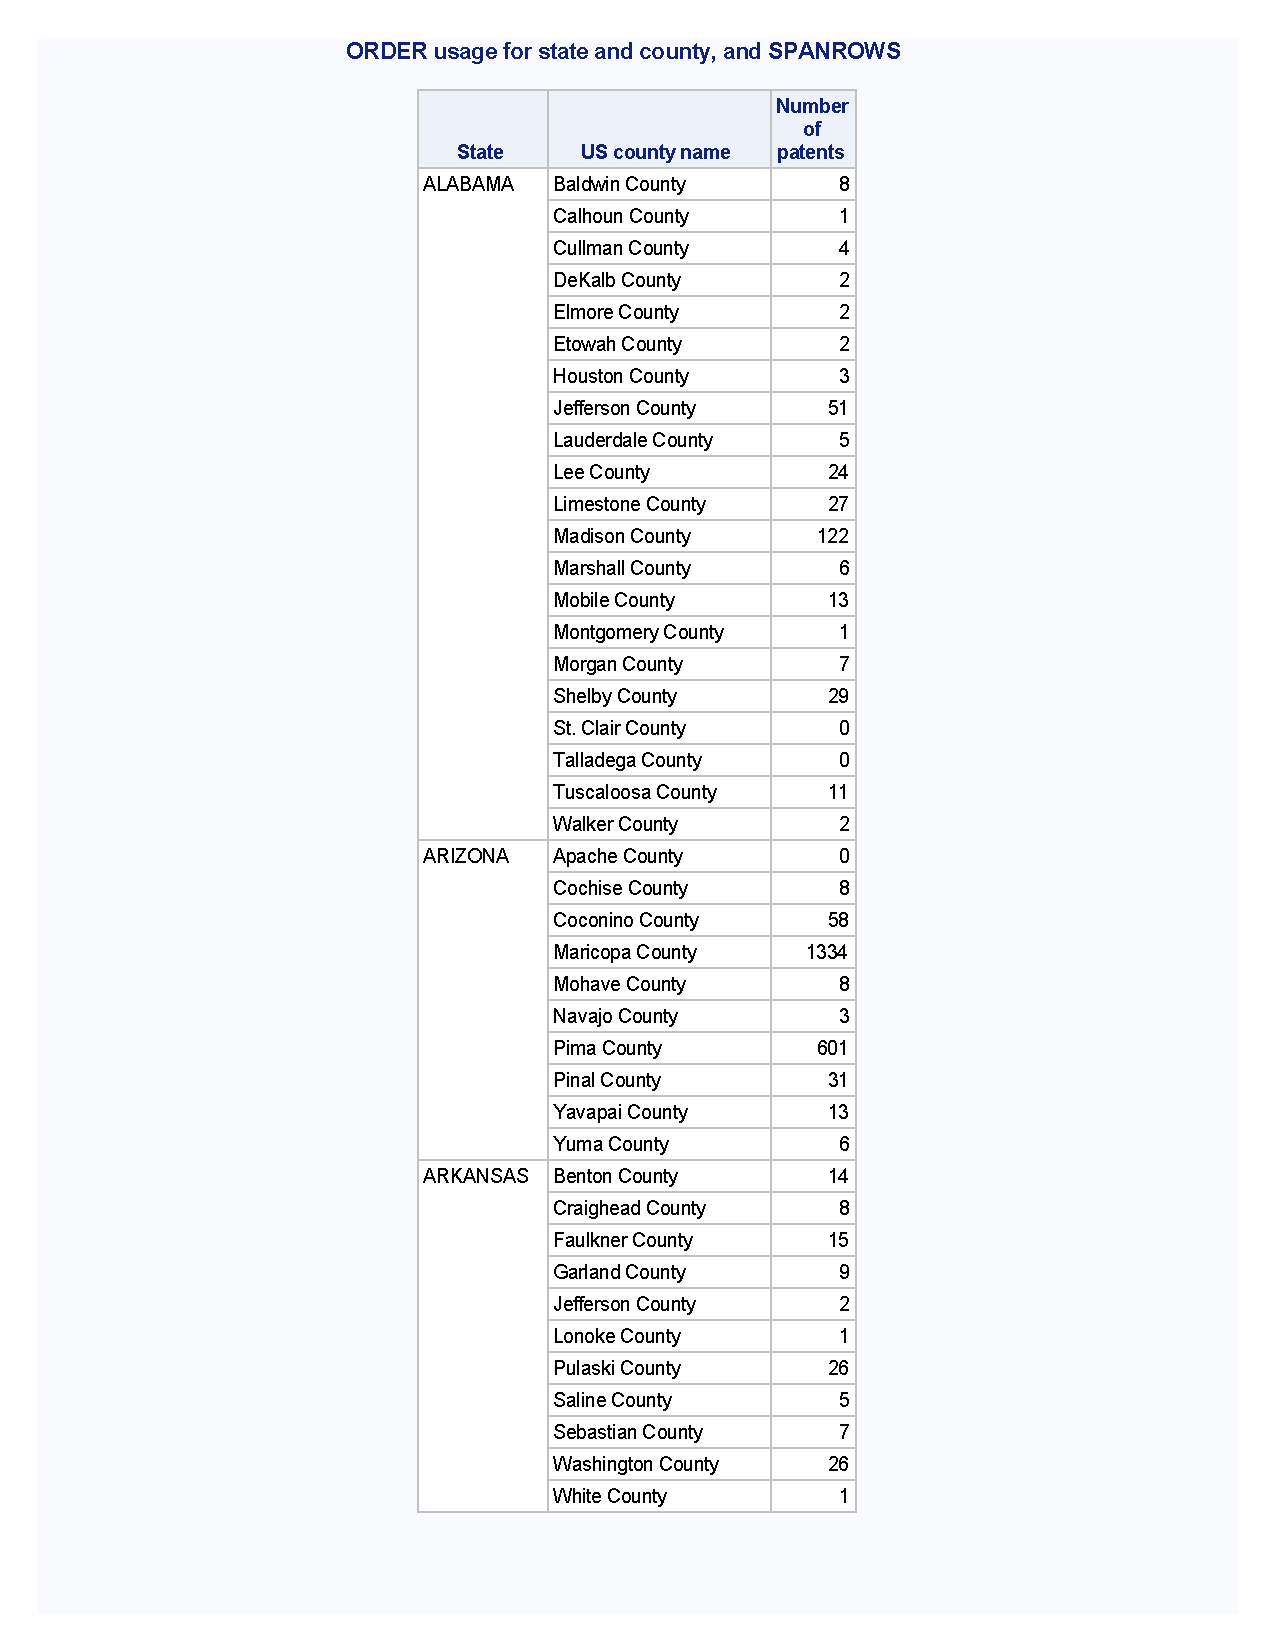
\includegraphics[trim={6.5cm 17.8cm 6.5cm 1.5cm},clip,width=1.0\textwidth]{L16_detail_order.pdf}
\emp
\end{frame}

\begin{frame}
\ft{Discussion}
\bmp{0.5\textwidth}
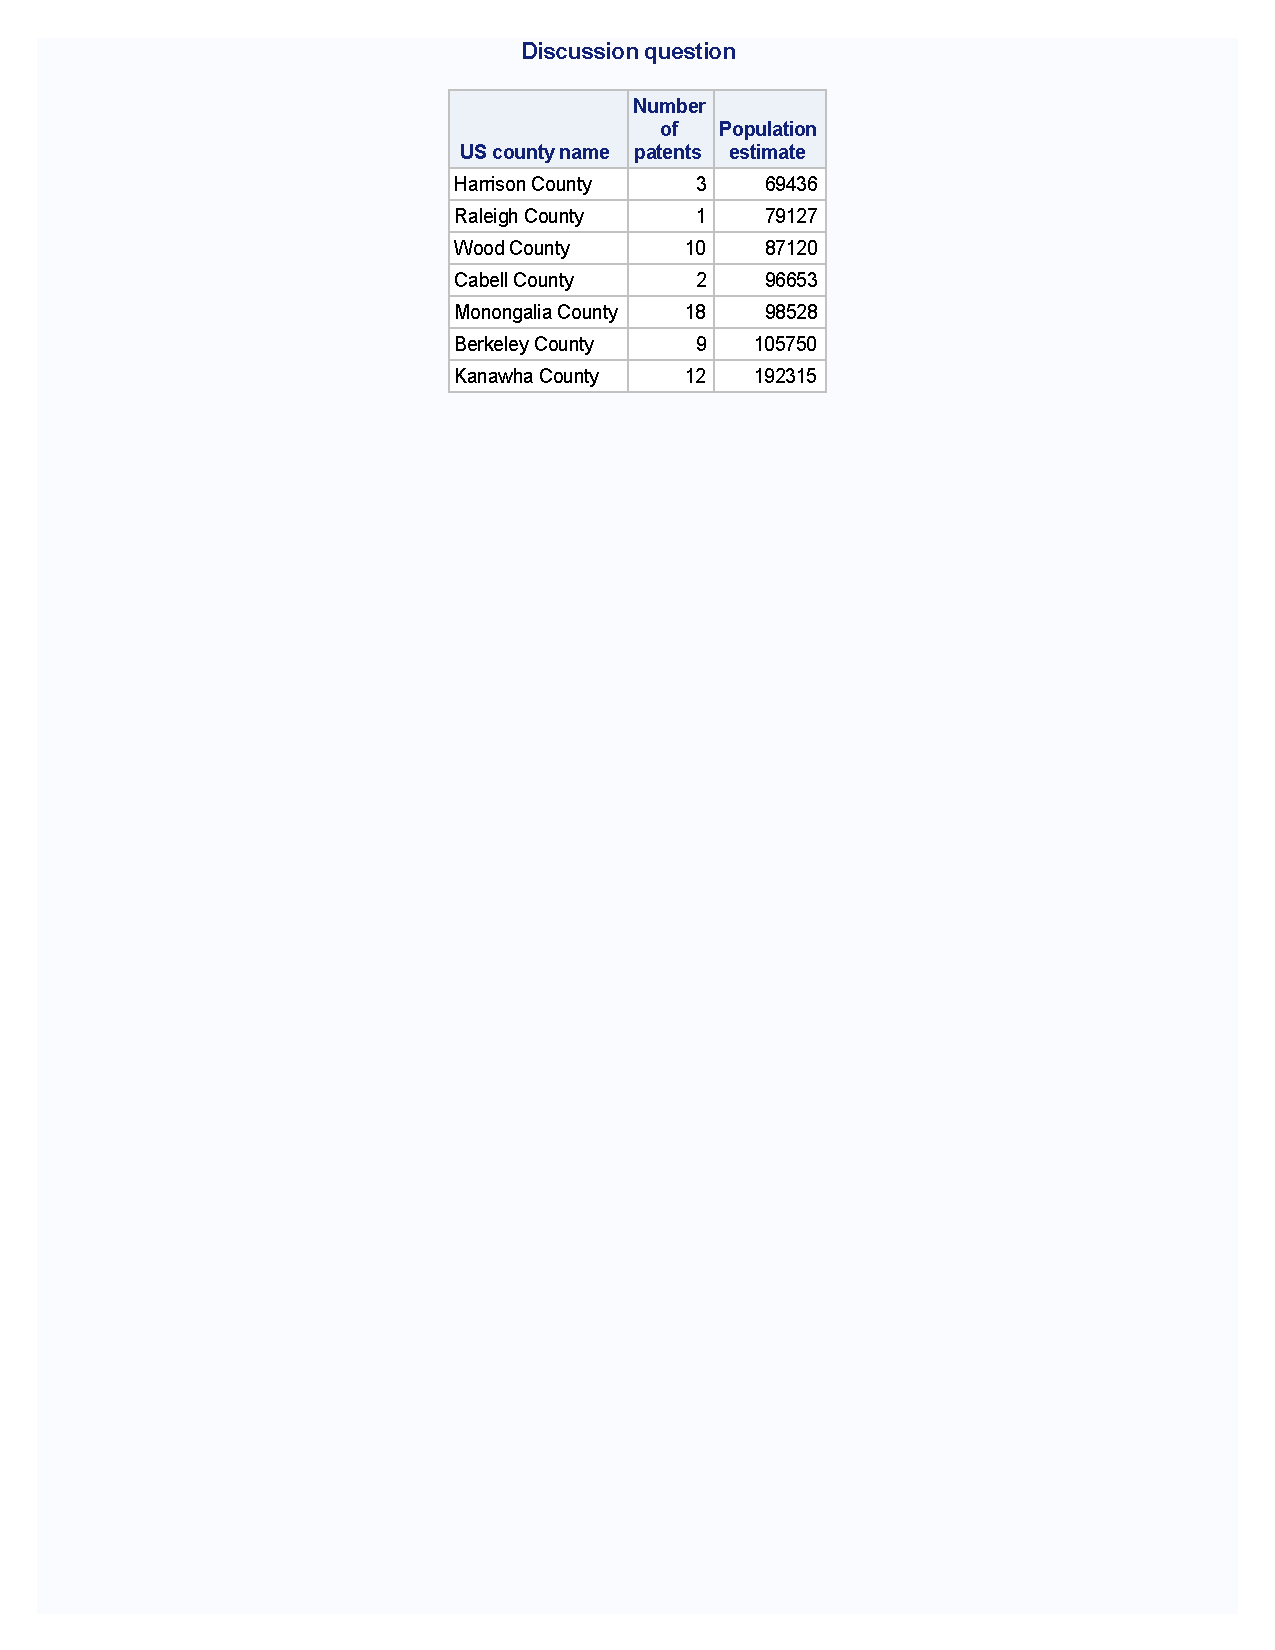
\includegraphics[trim={7.5cm 20cm 7.5cm 1.5cm},clip,width=1.0\textwidth]{L16_discussion1.pdf}
\emp
\bmp{0.05\textwidth} \hspace{0.05in} \emp
\bmp{0.45\textwidth}
\begin{clicker}{Identify the \emph{usage} of:}
\begin{enumerate}
\item \ttt{county}
\item[]
\item \ttt{patents}
\item[]
\item \ttt{population}
\item[]
\end{enumerate}
\end{clicker}
\emp
\end{frame}

\begin{frame}[fragile]
\ft{Discussion}
\hspace*{-0.3in}
\bmp{0.62\textwidth}
\begin{code}{.}
PROC REPORT DATA = patents  ;
   WHERE state = "ALABAMA" ;
   COLUMN county patents population;
   DEFINE county / DISPLAY ;
   DEFINE patents / ORDER ;
   DEFINE population / ANALYSIS ;
RUN ;
\end{code}
\vspace{10pt}
\oyo What do the blank values of \ttt{patents} represent?
\emp
\blankcolumn
\bmp{0.45\textwidth}
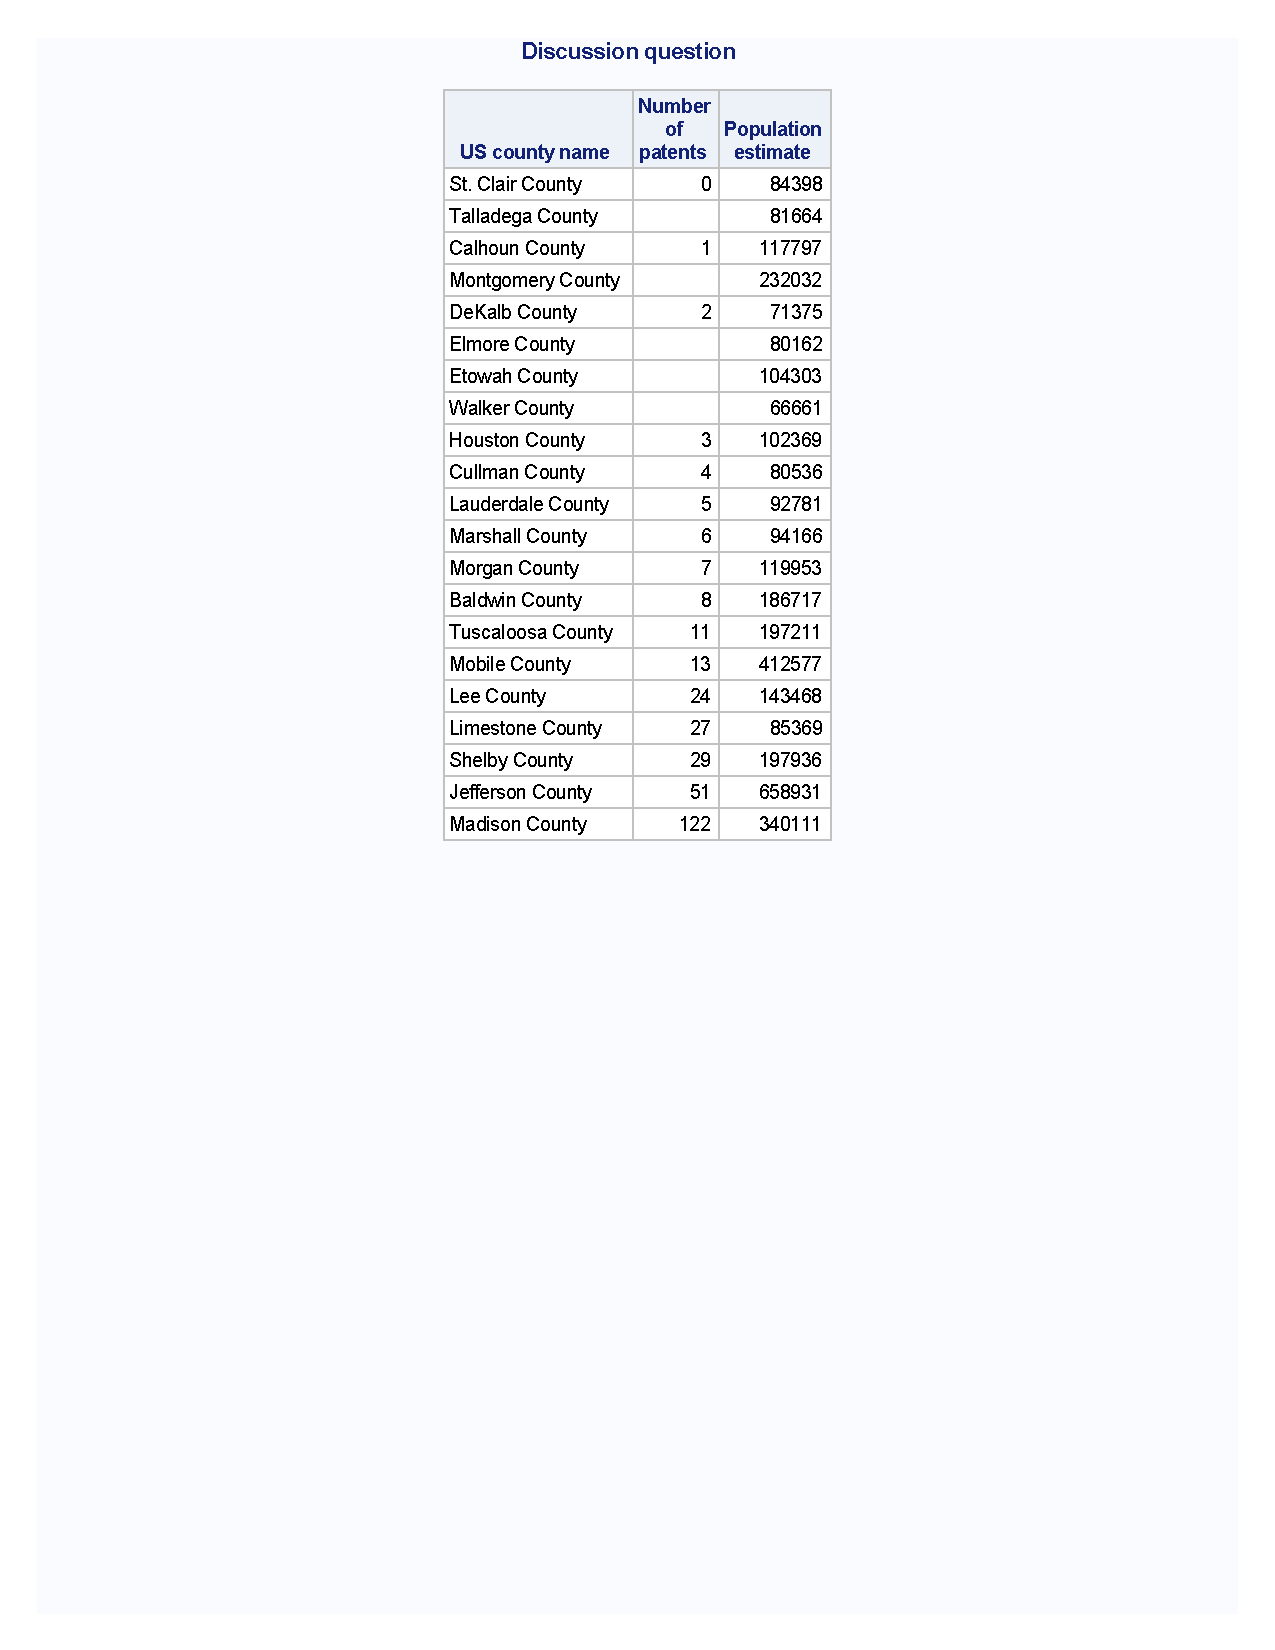
\includegraphics[trim={7.5cm 18cm 7.5cm 1.5cm},clip,width=1.0\textwidth]{L16_discussion2.pdf}
\emp

\end{frame}

\begin{frame}[fragile]
\ft{Spanning Column Headings}
\begin{center}
\fbox{\ttt{COLUMN ("\emph{header1}" \emph{items}) ("\emph{header2}" \emph{items}) }}
\end{center}
%\vskip10pt
\bmp{1.0\textwidth}
\begin{code}{.}
PROC REPORT DATA = patents SPANROWS;
  COLUMN \textcolor{OrangeRed}{("Location"} state county\textcolor{OrangeRed}{)}
         patents
         \textcolor{OrangeRed}{("Demographics"} population age education income\textcolor{OrangeRed}{)};
  DEFINE state / order;
  DEFINE county / order;
RUN;
\end{code}
\emp
\vspace{5pt}
%\begin{itemize}
%\item[]
%\item must use parentheses
%\item column header goes in quotes
%\item can also nest column headers
%\end{itemize}
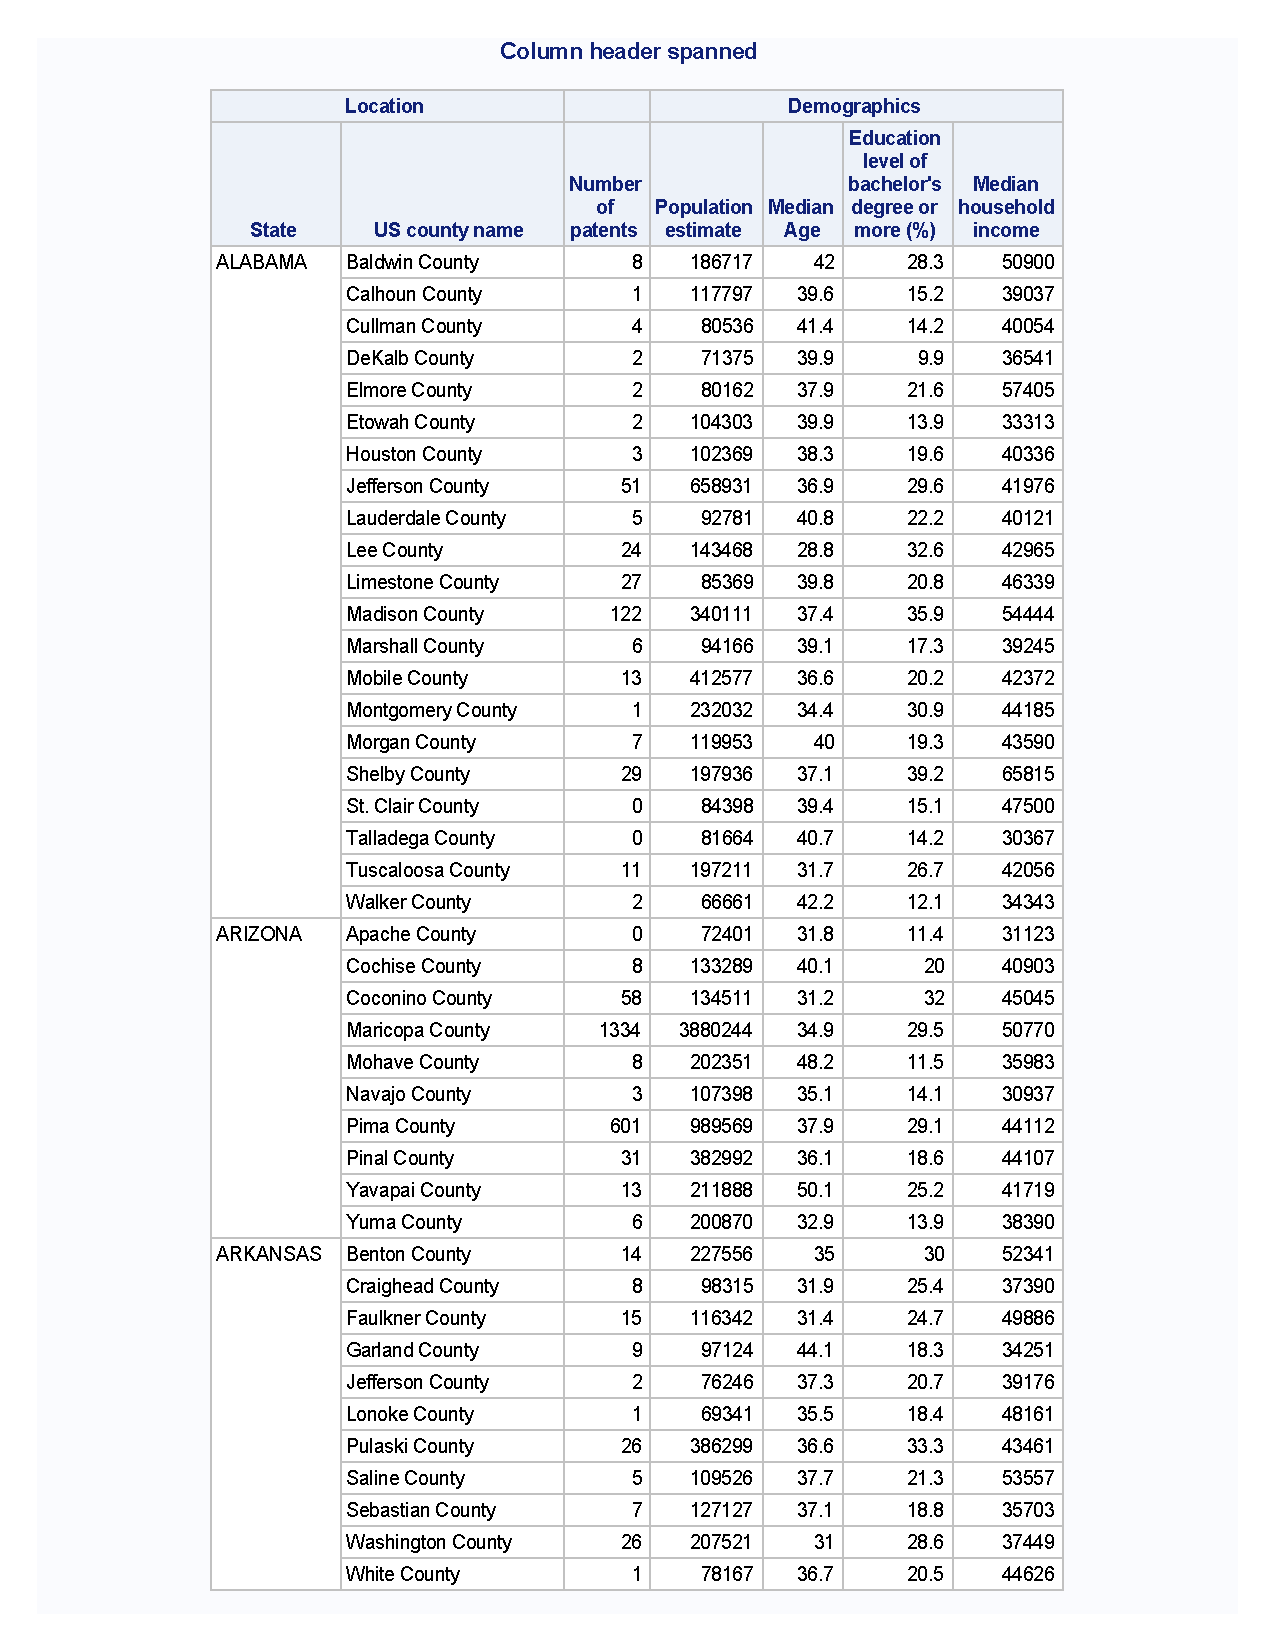
\includegraphics[trim={2.5cm 18cm 2.5cm 1.5cm},clip,width=1.0\textwidth]{L16_spancolhead.pdf}
\end{frame}

\begin{frame}[fragile]
\ft{Formats and Labels}
\begin{center}
\fbox{\ttt{DEFINE \emph{item} / F=\emph{myfmt.} "\emph{mylabel}" }}
\end{center}
%\vskip10pt
\bmp{1.1\textwidth}
\begin{code}{.}
PROC REPORT data=patents spanrows;
   COLUMN state county patents population age education income;
   DEFINE state / ORDER;
   DEFINE county / ORDER;
   DEFINE patents /  \textcolor{OrangeRed}{"Patents" F=COMMA15.} ;
   DEFINE population / \textcolor{OrangeRed}{"Population" F=COMMA15.} ;
   DEFINE education /  \textcolor{OrangeRed}{"\% >= Bachelor"} ;
   DEFINE income / \textcolor{OrangeRed}{F=DOLLAR15.} ;
RUN;
\end{code}
\emp
\vspace{5pt}
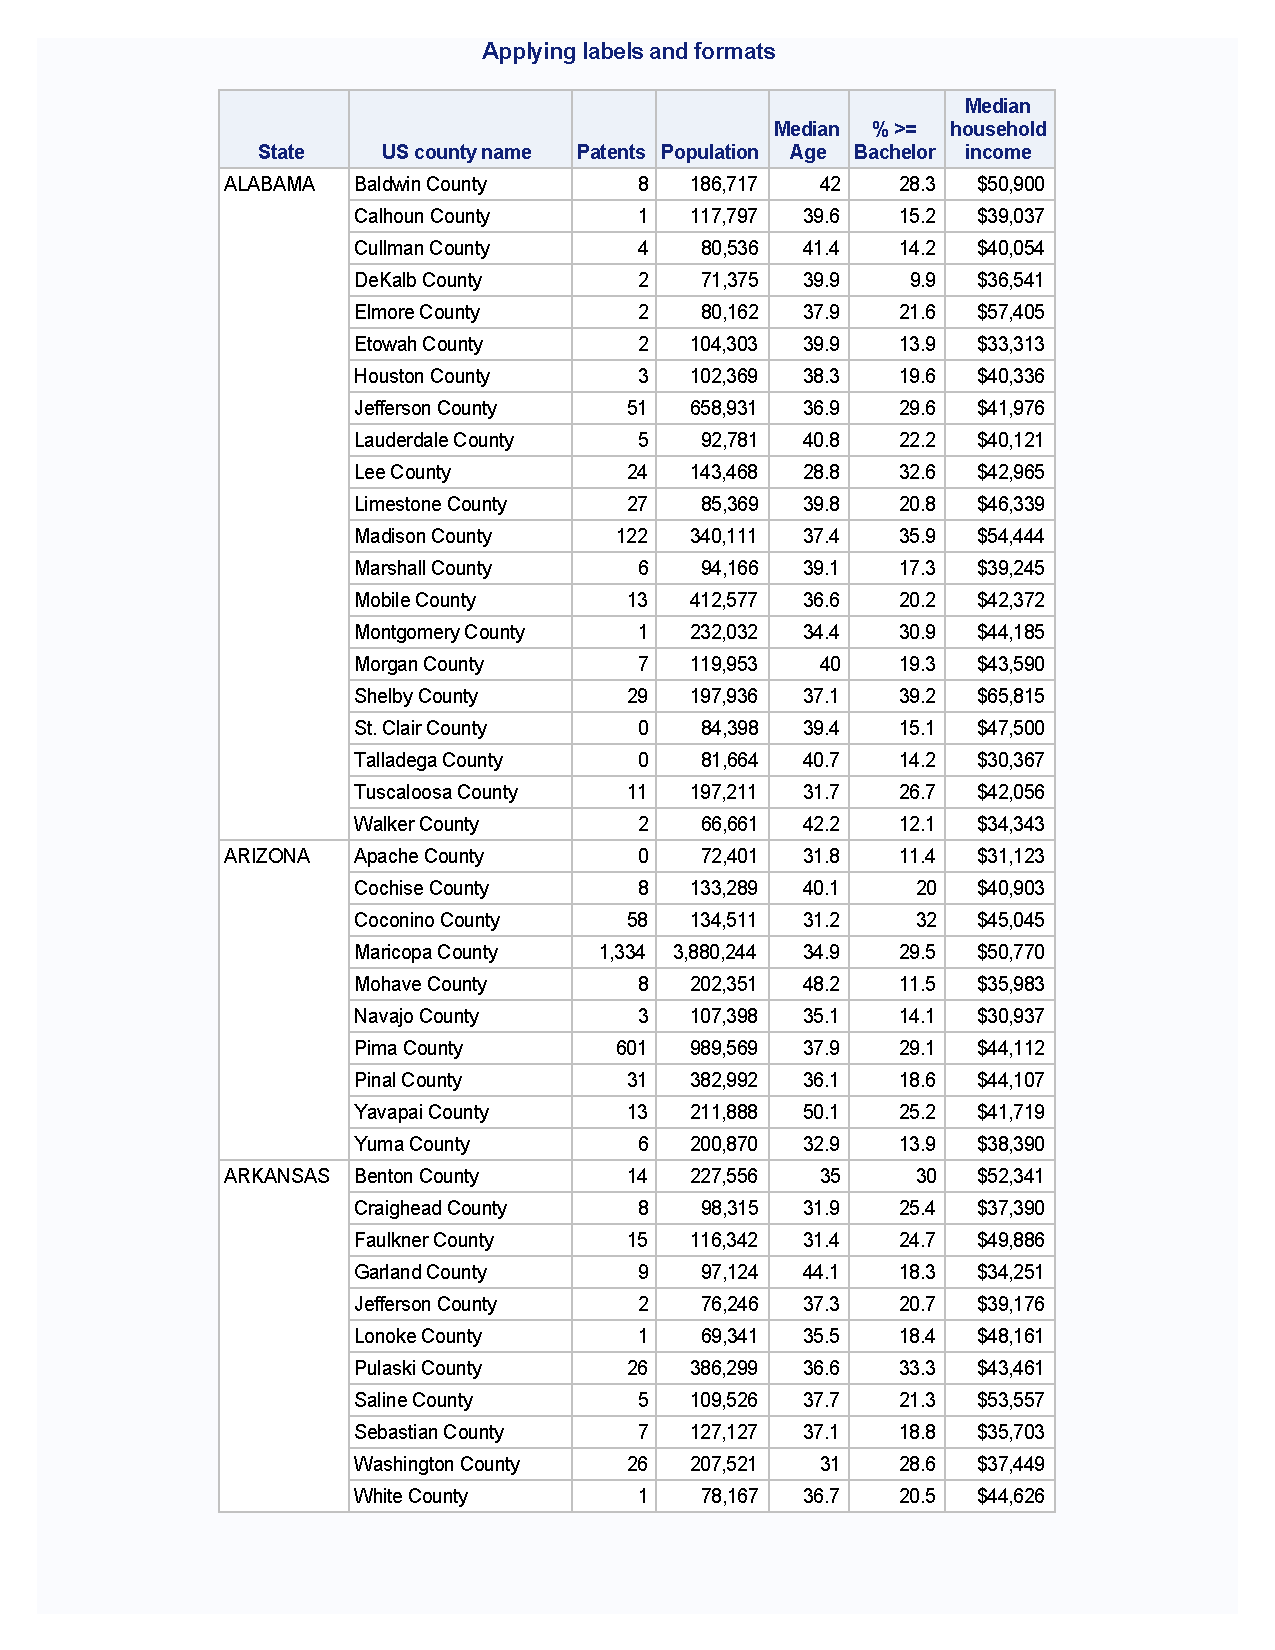
\includegraphics[trim={2.5cm 18cm 2.5cm 1.5cm},clip,width=1.0\textwidth]{L16_format_label.pdf}
\end{frame}

%===========================================================================================================================
\section[Summary Report with GROUP]{Summary Report with GROUP}
%===========================================================================================================================
\subsection{}
\begin{frame}
\tableofcontents[currentsection, hideallsubsections]
\end{frame}

\begin{frame}[fragile]
\ft{GROUP example}
\bmp{0.62\textwidth}
\begin{code}{.}
PROC REPORT DATA = patents SPANROWS ;
   COLUMN region division patents  ;
   DEFINE region / \textcolor{OrangeRed}{GROUP};
   DEFINE division / \textcolor{OrangeRed}{GROUP};
RUN;
\end{code}
\emp
\blankcolumn
\bmp{0.4\textwidth}
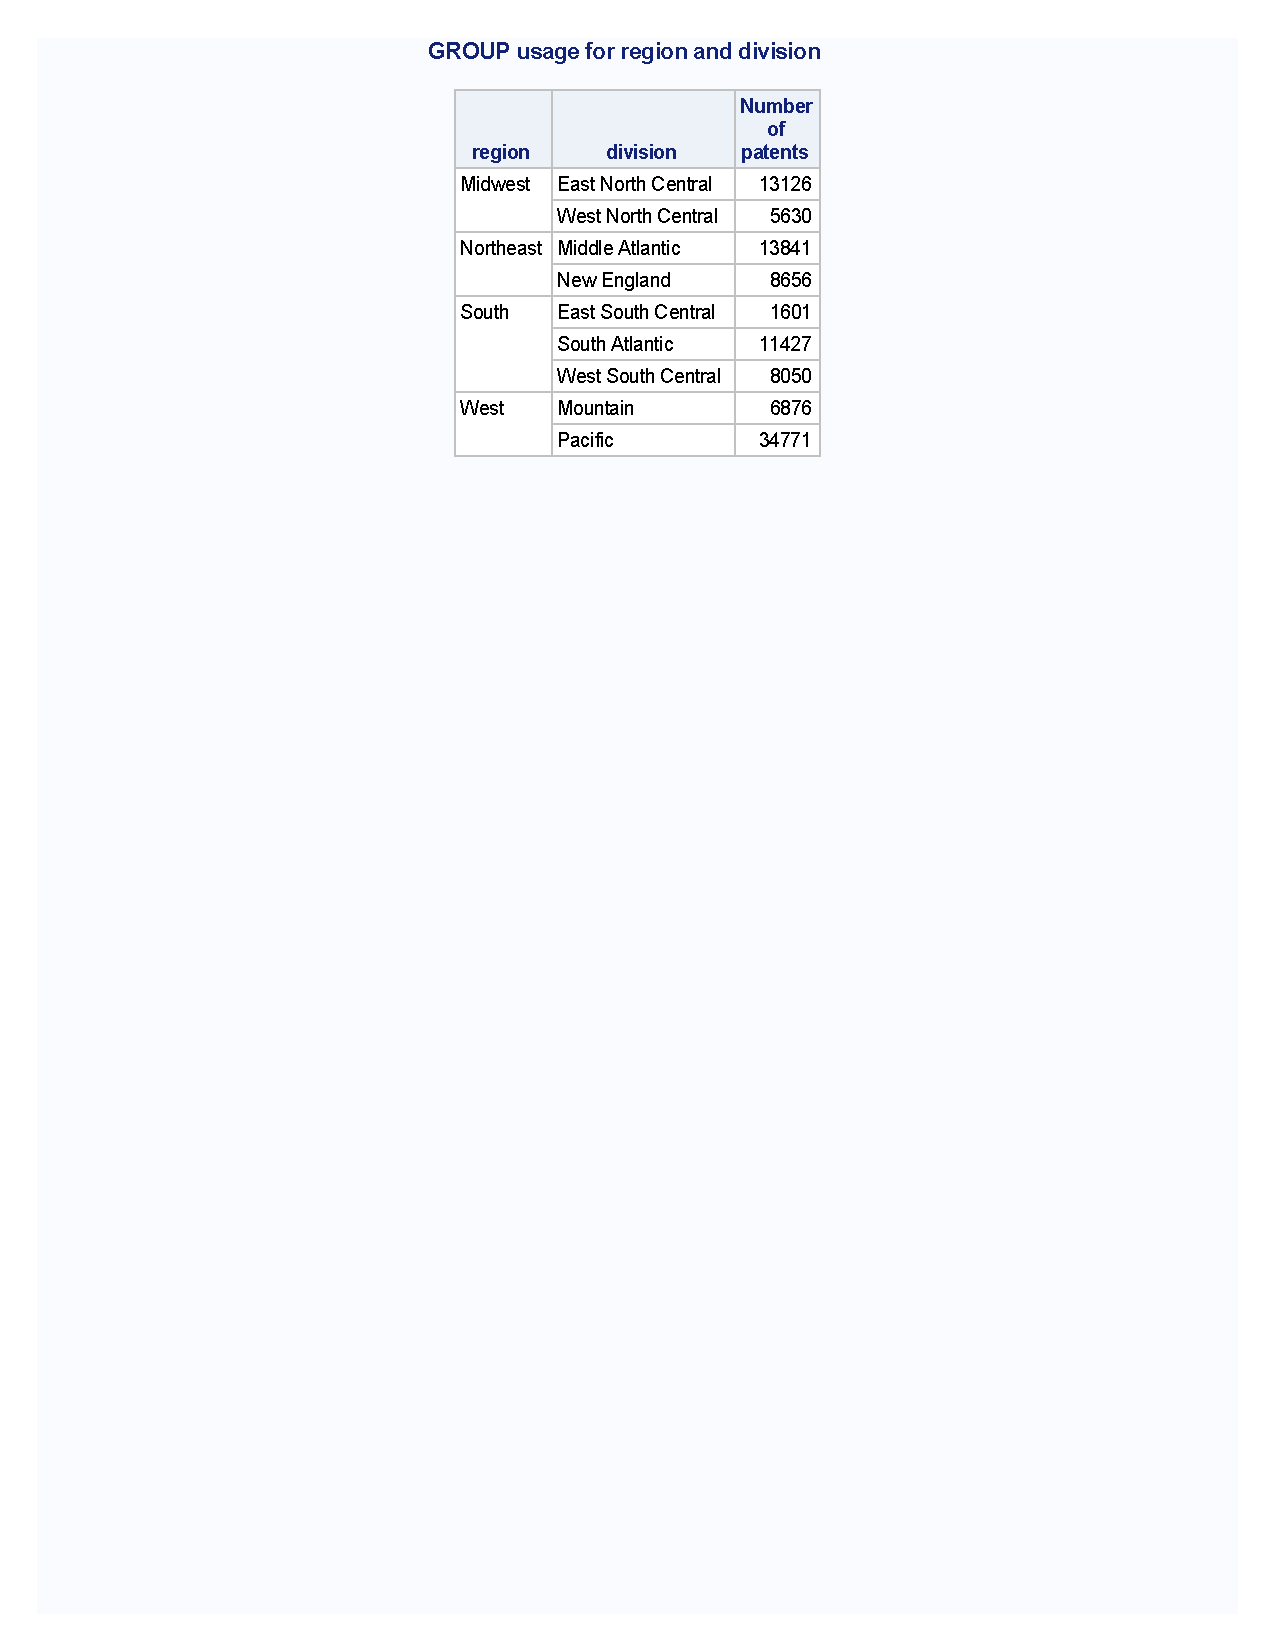
\includegraphics[trim={7.5cm 20cm 7.5cm 1.5cm},clip,width=1.0\textwidth]{L16_group.pdf}
\emp
\vskip10pt
\underline{\ttt{GROUP} usage}
\bi
\item \emph{summarizes} data
\item collapses observations with same values
\item places values on rows
\item orders rows
\item suppresses repetitious printing
\ei
\end{frame}

\begin{frame}[fragile]
\ft{Default statistics}
Defaults for numeric variables:
\bi
\item \ttt{ANALYSIS} usage
\item \ttt{SUM} statistic
\item[]
\ei
\bmp{0.75\textwidth}
\begin{craw}{.}{Equivalent Statements}
DEFINE patents / "Patents";

DEFINE patents / ANALYSIS "Patents";

DEFINE patents / ANALYSIS SUM "Patents";

DEFINE patents / SUM "Patents";
\end{craw}
\emp
\end{frame}

\begin{frame}
\ft{Statistics keywords}
\begin{center}
\resizebox{1.0\textwidth}{!}{
\begin{tabular}{lllll}
CSS & CV & MAX & MEAN & MIN \\
MODE & N & NMISS & RANGE & STDEV \\
STDERR & SUM & SUMWGT &  USS & VAR \\
PCTN & PCTSUM \\
MEDIAN$|$P50 & P1 & P5 & P10 & P25$|$Q1  \\
P75$|$Q3 & P90 & P95 & P99 & QRANGE  \\
\end{tabular}}
\end{center}
\end{frame}


\begin{frame}[fragile]
\ft{Specifying statistics}
\bmp{1.0\textwidth}
\begin{code}{.}
PROC REPORT DATA = patents SPANROWS;
   COLUMN region division \textcolor{OrangeRed}{N PCTN} patents,(\textcolor{OrangeRed}{SUM MEAN}) income ;
   DEFINE region / GROUP;
   DEFINE division / GROUP;
   DEFINE patents / ANALYSIS "Patents" ;
   DEFINE income / ANALYSIS \textcolor{OrangeRed}{MEAN} "Ave Income" F=DOLLAR10. ;
   DEFINE \textcolor{OrangeRed}{PCTN} / "Percent" F=PERCENT8.1;
   DEFINE \textcolor{OrangeRed}{MEAN} / "Mean" F=COMMA10.1;
   DEFINE \textcolor{OrangeRed}{SUM} / "Sum" F=COMMA10.;
RUN;
\end{code}
\emp
\bi
\item \ttt{N} and \ttt{PCTN} can be specified \ttt{COLUMN} statement
\item All other statistics must be associated with a numeric variable
\bi
\item Single statistic: specify in \ttt{DEFINE}
\item Multiple statistics: specify with comma in \ttt{COLUMN}
\ei
\ei
\end{frame}

\begin{frame}[fragile]
\ft{Specifying statistics, example output}
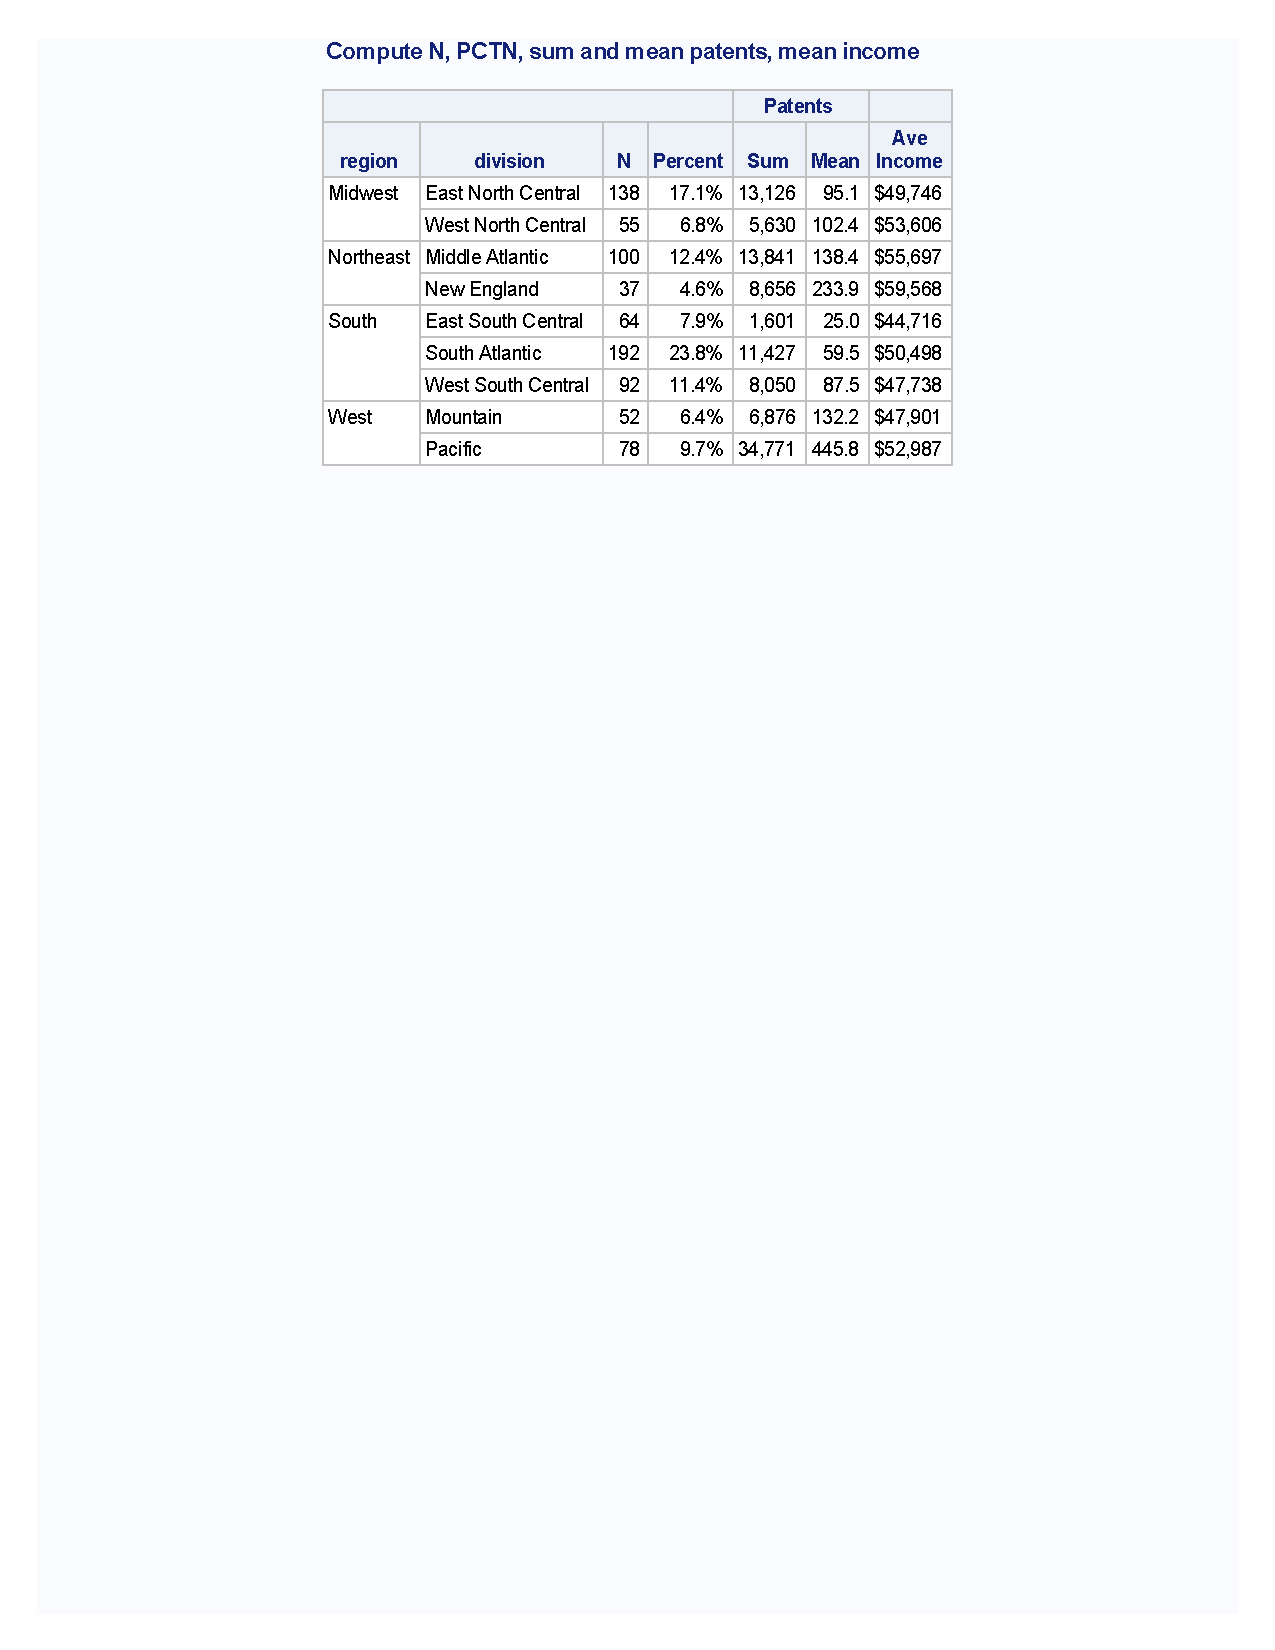
\includegraphics[trim={4.5cm 20cm 4.5cm 1.5cm},clip,width=0.80\textwidth]{L16_stats.pdf}
\end{frame}

%===========================================================================================================================
\section[Summary Report with ACROSS]{Summary Report with ACROSS}
%===========================================================================================================================
\subsection{}
\begin{frame}
\tableofcontents[currentsection, hideallsubsections]
\end{frame}



\begin{frame}[fragile]
\ft{ACROSS example}
\hspace*{-0.3in}
\bmp{0.73\textwidth}
\begin{code}{.}
PROC REPORT DATA = patents SPANROWS;
   COLUMN region division N edu25 patents ;
   DEFINE region / GROUP;
   DEFINE division / GROUP;
   DEFINE edu25 / \textcolor{OrangeRed}{ACROSS};
   DEFINE patents / "Patents" F=COMMA15.;
RUN;
\end{code}
\emp
\blankcolumn
\bmp{0.32\textwidth}
\underline{\ttt{ACROSS} usage}
\bi
\item \emph{summarizes} data
\item collapses observations with same values
\item places ordered values on columns
\item default statistic is \ttt{N}
\ei
\emp
\vspace{5pt}
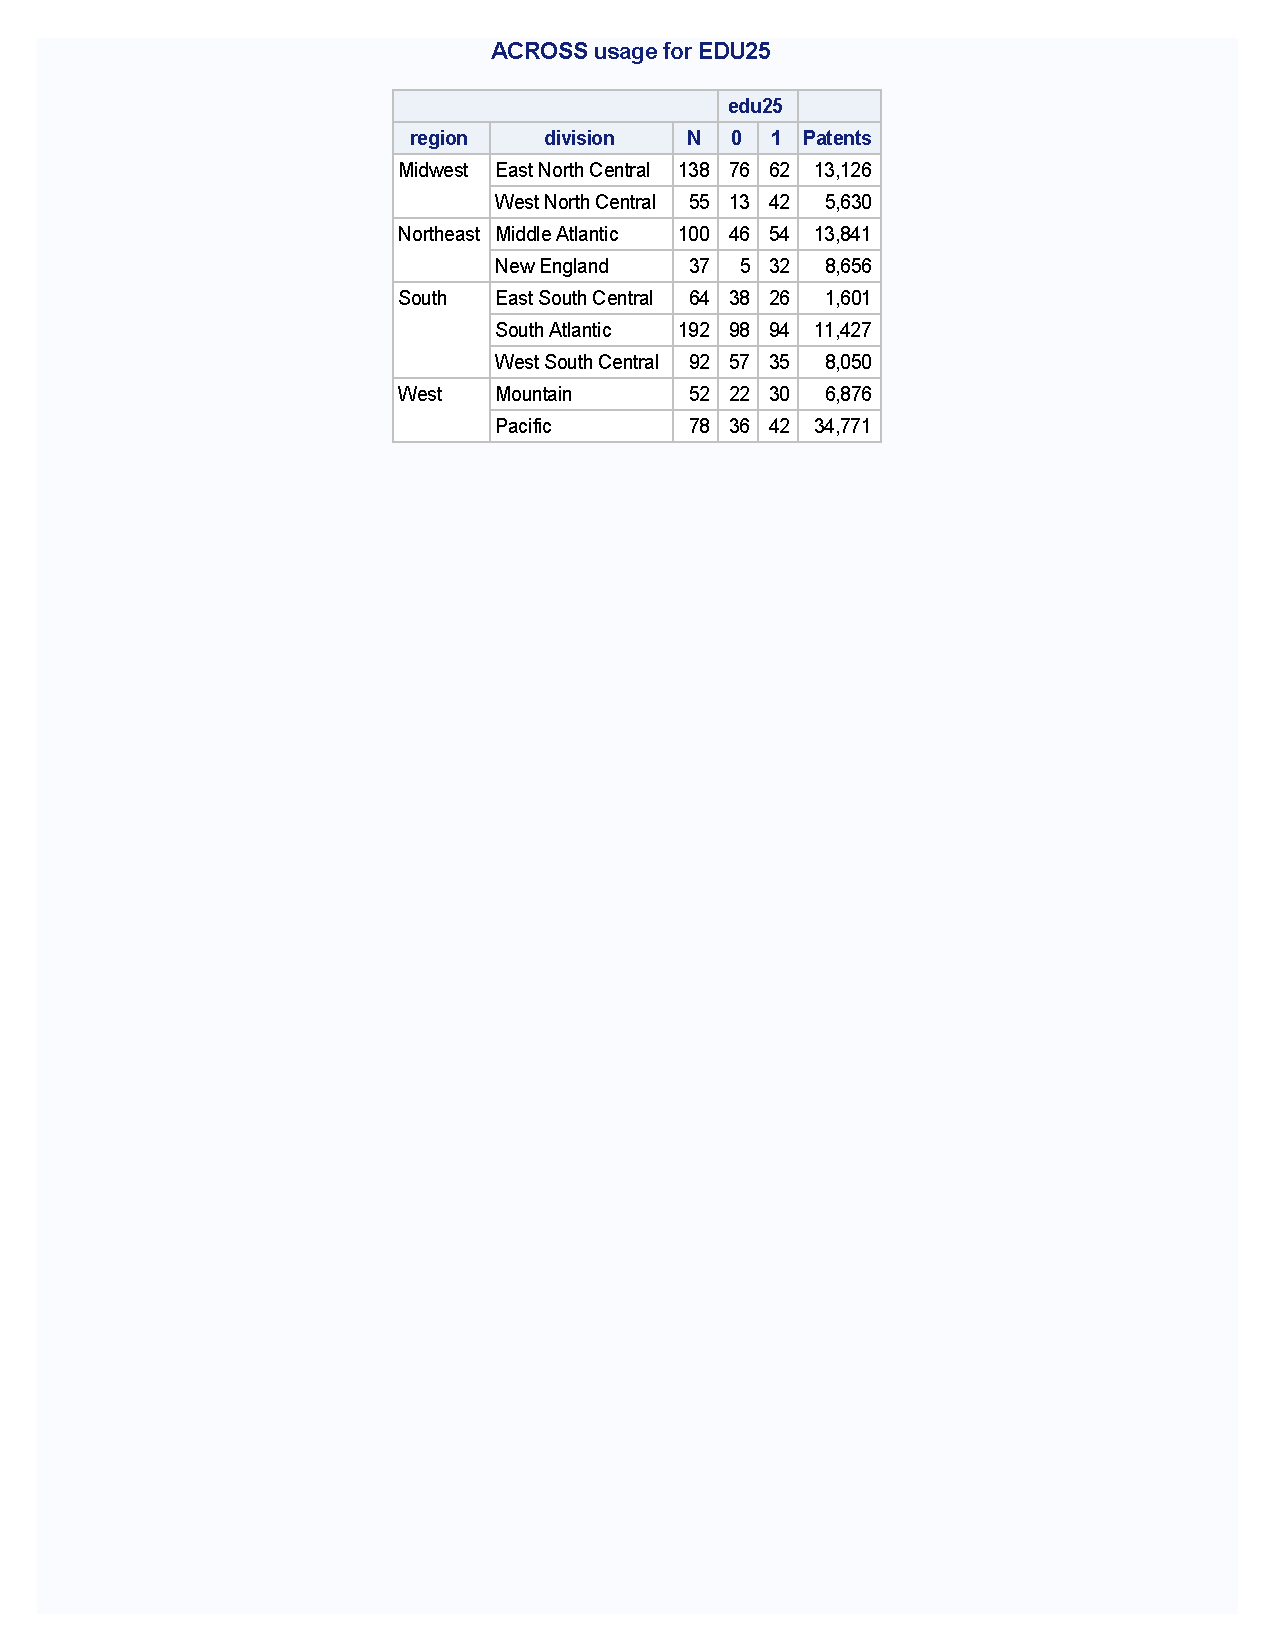
\includegraphics[trim={5.5cm 20cm 5.5cm 1.5cm},clip,width=0.70\textwidth]{L16_across.pdf}
\end{frame}


\begin{frame}[fragile]
\ft{Analysis variables within ACROSS}
\hspace*{-0.3in}
\bmp{0.71\textwidth}
\begin{code}{.}
PROC REPORT DATA = patents SPANROWS;
   COLUMN region division N \textcolor{OrangeRed}{edu25,patents};
   DEFINE region / GROUP;
   DEFINE division / GROUP;
   DEFINE edu25 / ACROSS;
   DEFINE patents /  F=COMMA15.;
RUN;
\end{code}
\begin{code}{.}
PROC REPORT DATA = patents SPANROWS;
   COLUMN region division N \textcolor{OrangeRed}{patents,edu25};
   DEFINE region / GROUP;
   DEFINE division / GROUP;
   DEFINE edu25 / ACROSS;
   DEFINE patents / " " F=COMMA15.;
RUN;
\end{code}
\emp
\blankcolumn
\bmp{0.35\textwidth}
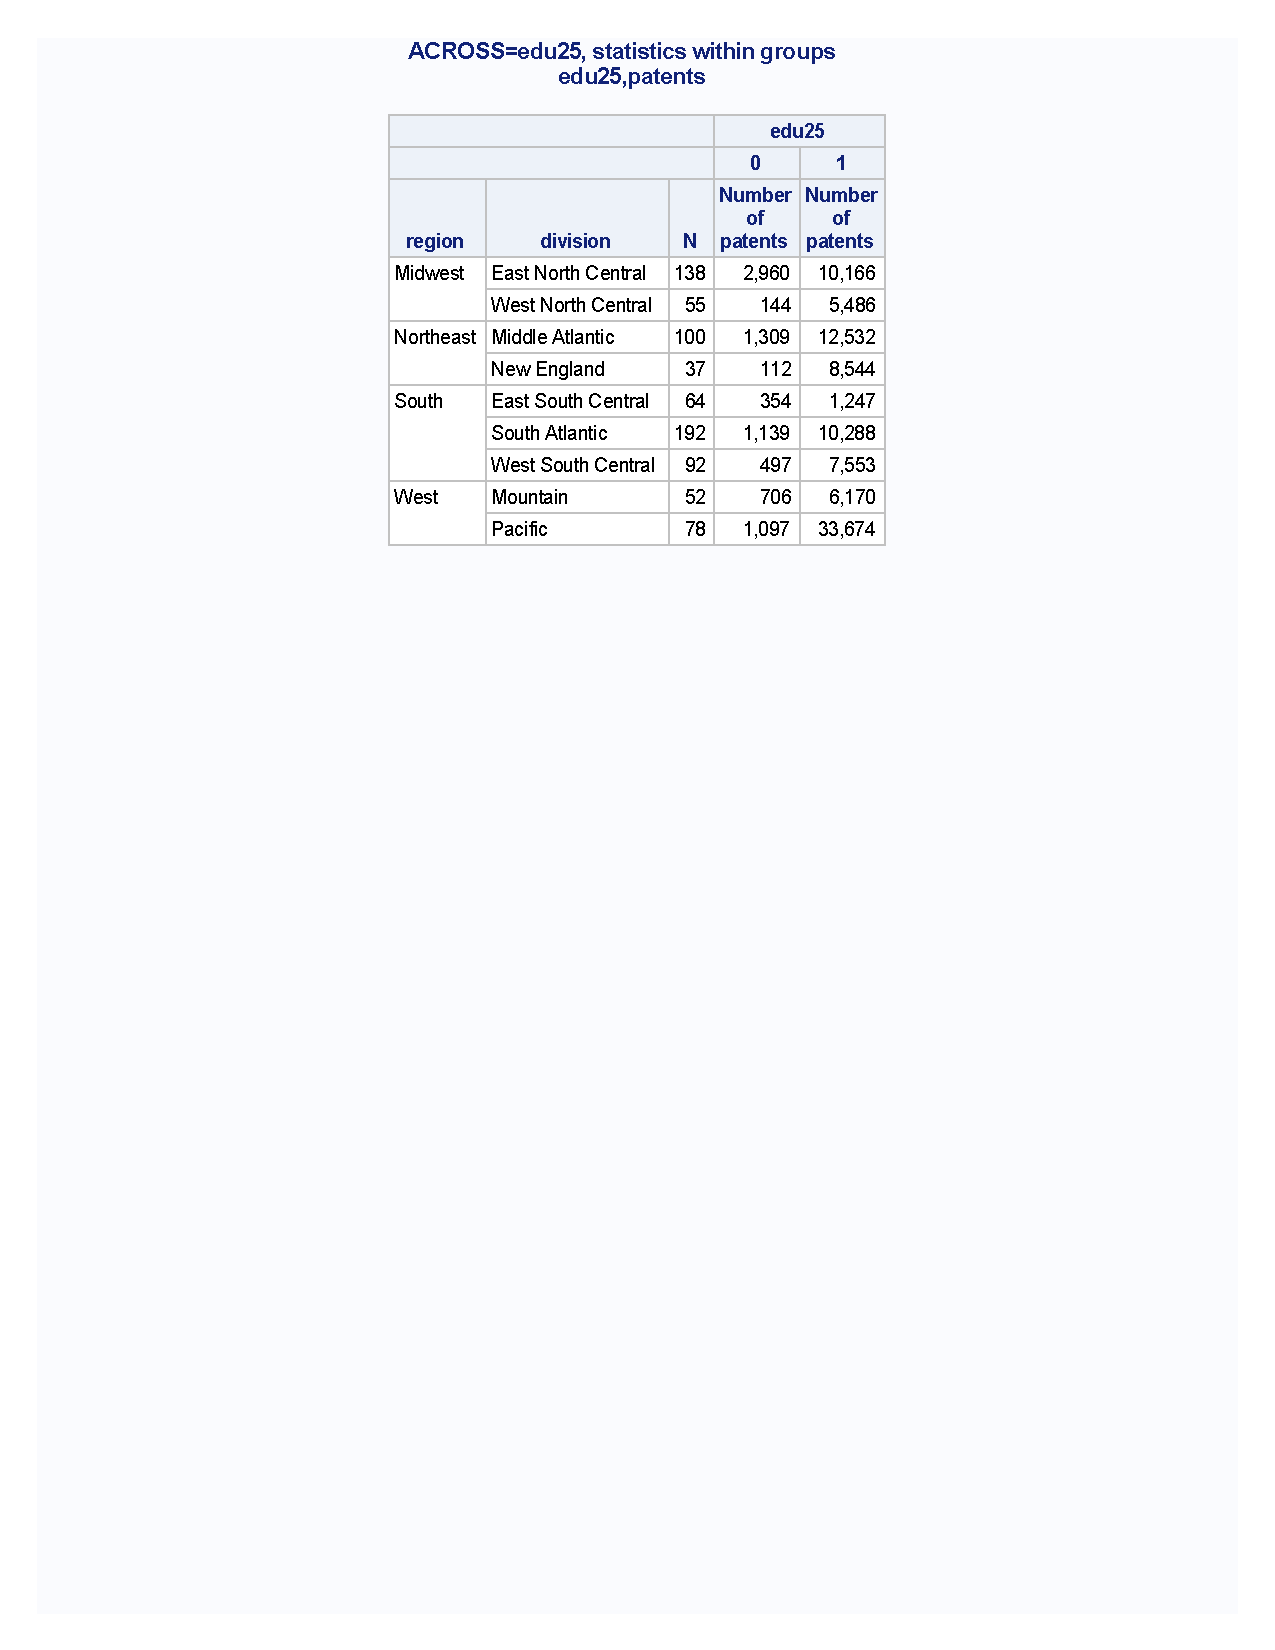
\includegraphics[trim={6cm 18.5cm 6cm 1.5cm},clip,width=1.0\textwidth]{L16_across_nest1.pdf}\\
\vskip25pt
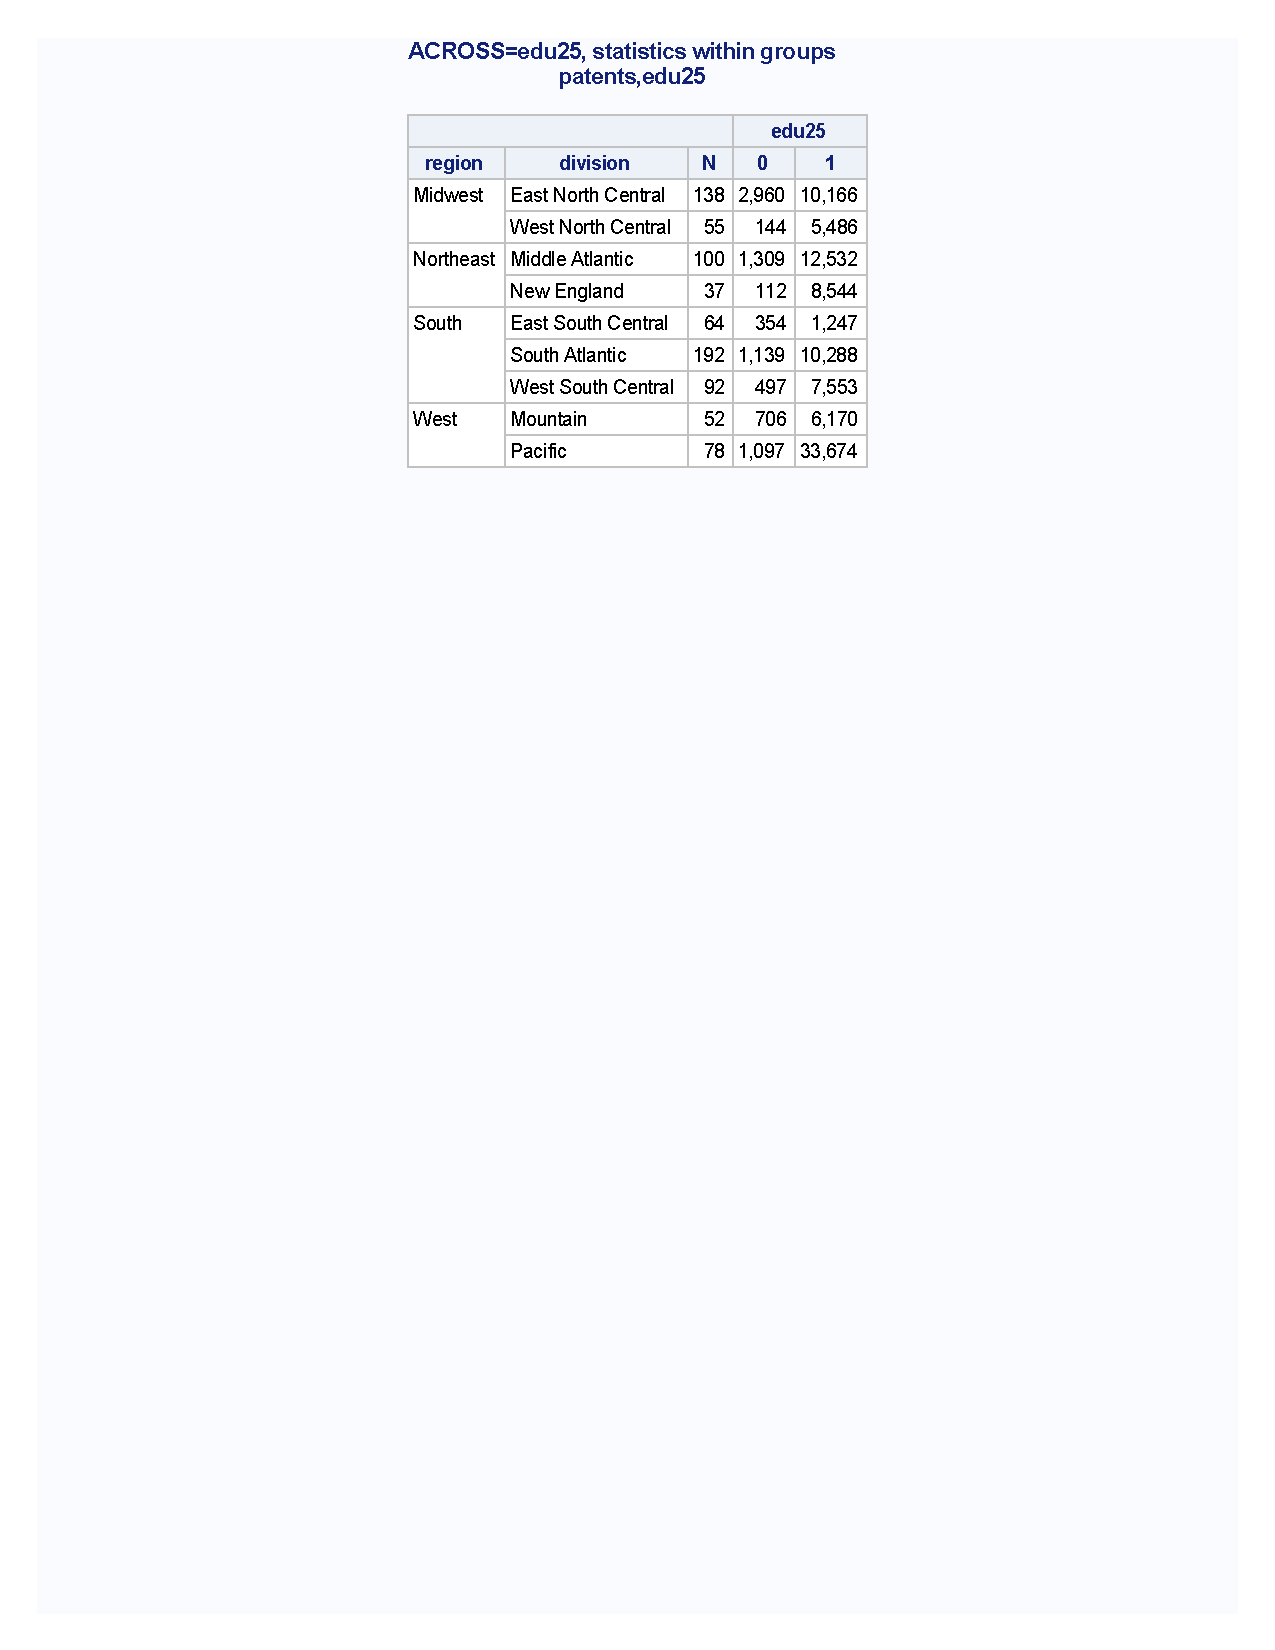
\includegraphics[trim={6cm 19cm 6cm 1.5cm},clip,width=1.0\textwidth]{L16_across_nest2.pdf}
\emp
\end{frame}

\begin{frame}[fragile]
\ft{Multiple analysis variables within ACROSS}
\bmp{0.85\textwidth}
\begin{code}{.}
PROC REPORT DATA = patents SPANROWS;
   COLUMN region division N \textcolor{OrangeRed}{edu25,(patents income)};
   DEFINE region / GROUP;
   DEFINE division / GROUP;
   DEFINE edu25 / ACROSS;
   DEFINE patents / "Patents" SUM  F=COMMA15.;
   DEFINE income /  "Income" MEAN F=DOLLAR15.;
RUN;
\end{code}
\emp
\vspace{5pt}
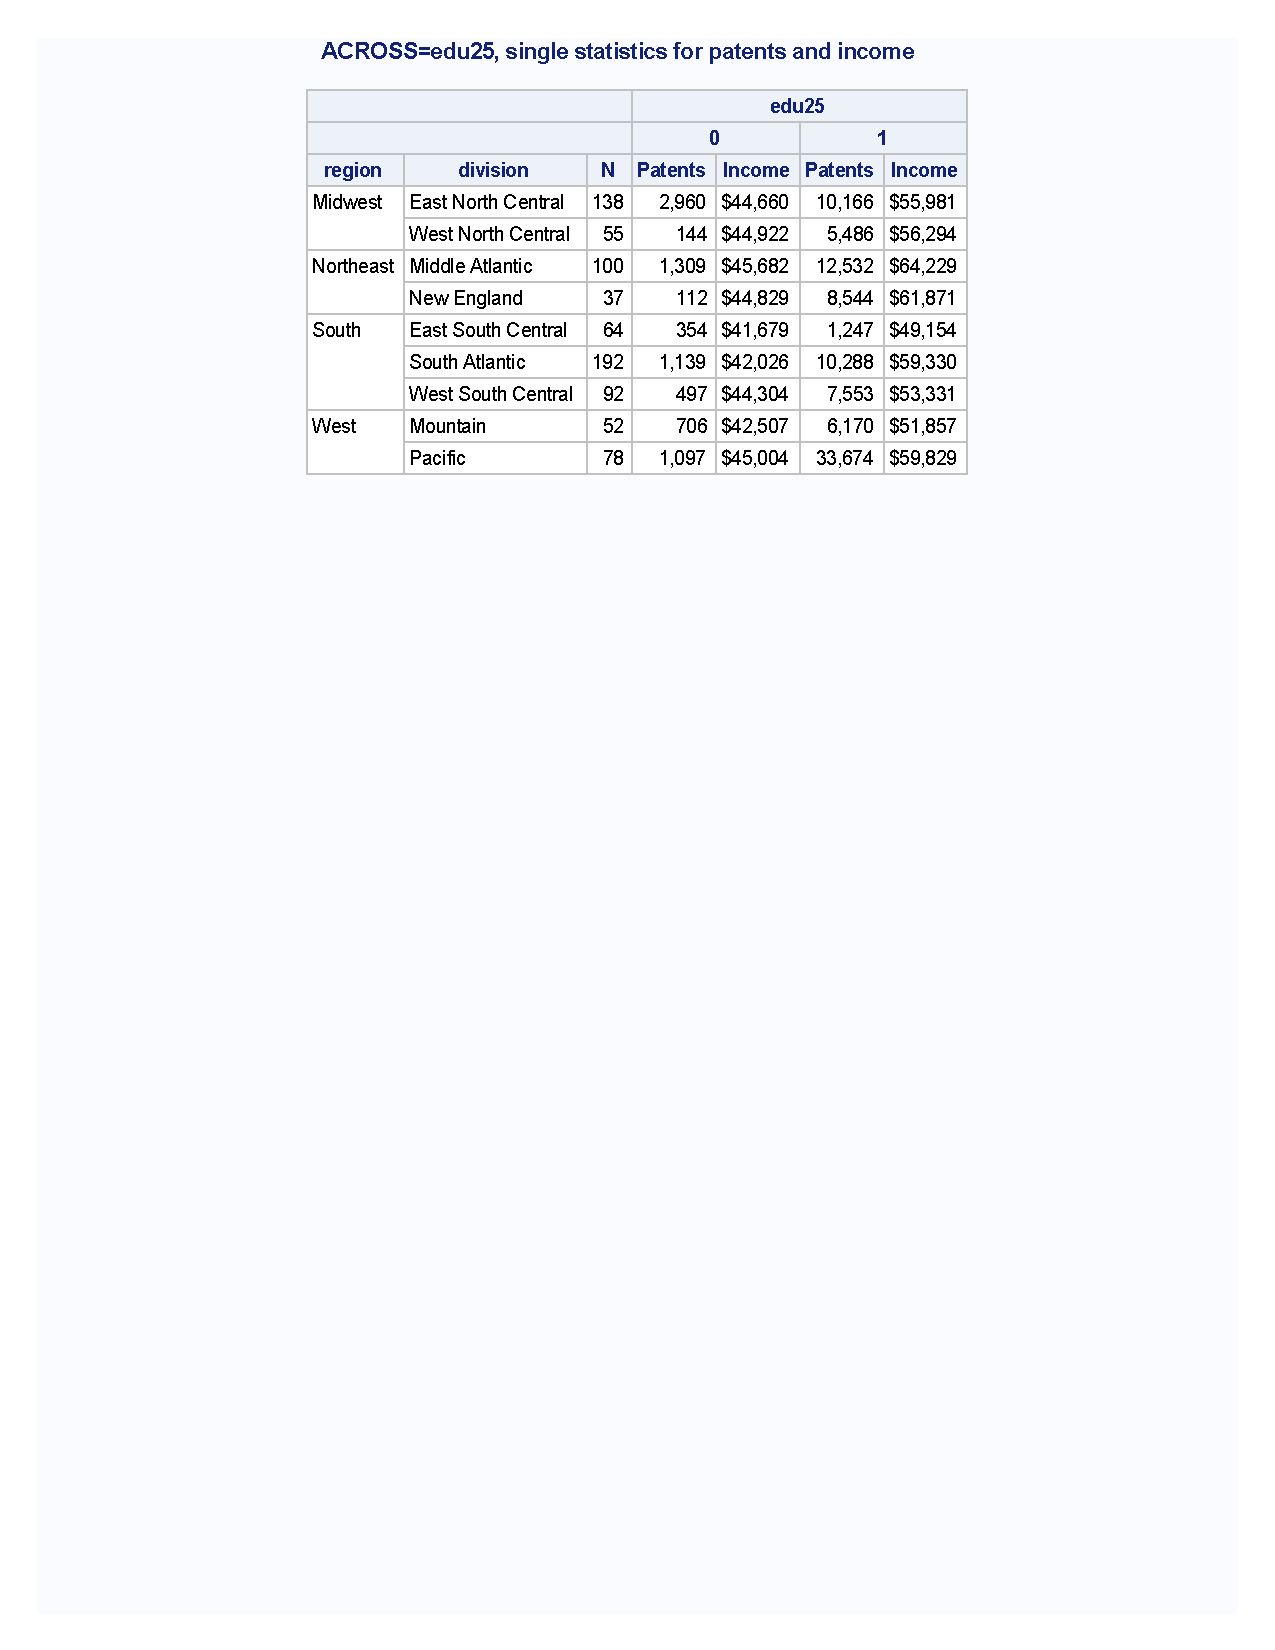
\includegraphics[trim={4.5cm 19cm 4.5cm 1.5cm},clip,width=0.9\textwidth]{L16_across_multnest.pdf}\\
\end{frame}


%\begin{frame}[fragile]
%\ft{Analysis variables within ACROSS}
%Use comma to nest an analysis variable within an across variable: \\
%\vskip5pt
%\fbox{\ttt{COLUMN \emph{AcrossVar}, \emph{AnalysisVar};}} \\
%\vskip5pt
%\fbox{\ttt{COLUMN \emph{AnalysisVar}, \emph{AcrossVar};}} (streamlines  headings)\\
%\vskip20pt
%Use comma and parentheses to nest multiple analysis variables with an across variable:\\
%\vskip5pt
%\fbox{\ttt{COLUMN \emph{AcrossVar}, (\emph{AnalysisVar1} \emph{AnalysisVar2});}}\\
%\vskip20pt
%\oyo Which statistic will be calculated for \emph{AnalysisVar1} and \emph{AnalysisVar2} unless otherwise specified?  How could you change that?
%\end{frame}

\begin{frame}[fragile]
\ft{Multiple statistics for analysis variables within ACROSS}
\hspace*{-0.3in}
\bmp{1.1\textwidth}
Use commas and parentheses to nest multiple statistics for an analysis variable within an across variable:\\
\vskip5pt
\fbox{\ttt{COLUMN \emph{AcrossVar},\emph{AnalysisVar},(\emph{stat1} \emph{stat2});}}
\vskip30pt
Use commas and parentheses to nest multiple statistics for multiple analysis variables within an across variable:\\
\vskip5pt
\fbox{\ttt{COLUMN \emph{AcrossVar},(\emph{AnalysisVar1} \emph{AnalysisVar2}),(\emph{stat1} \emph{stat2});}}
\emp
\end{frame}

\begin{frame}[fragile]
\ft{Discussion}
\begin{center}
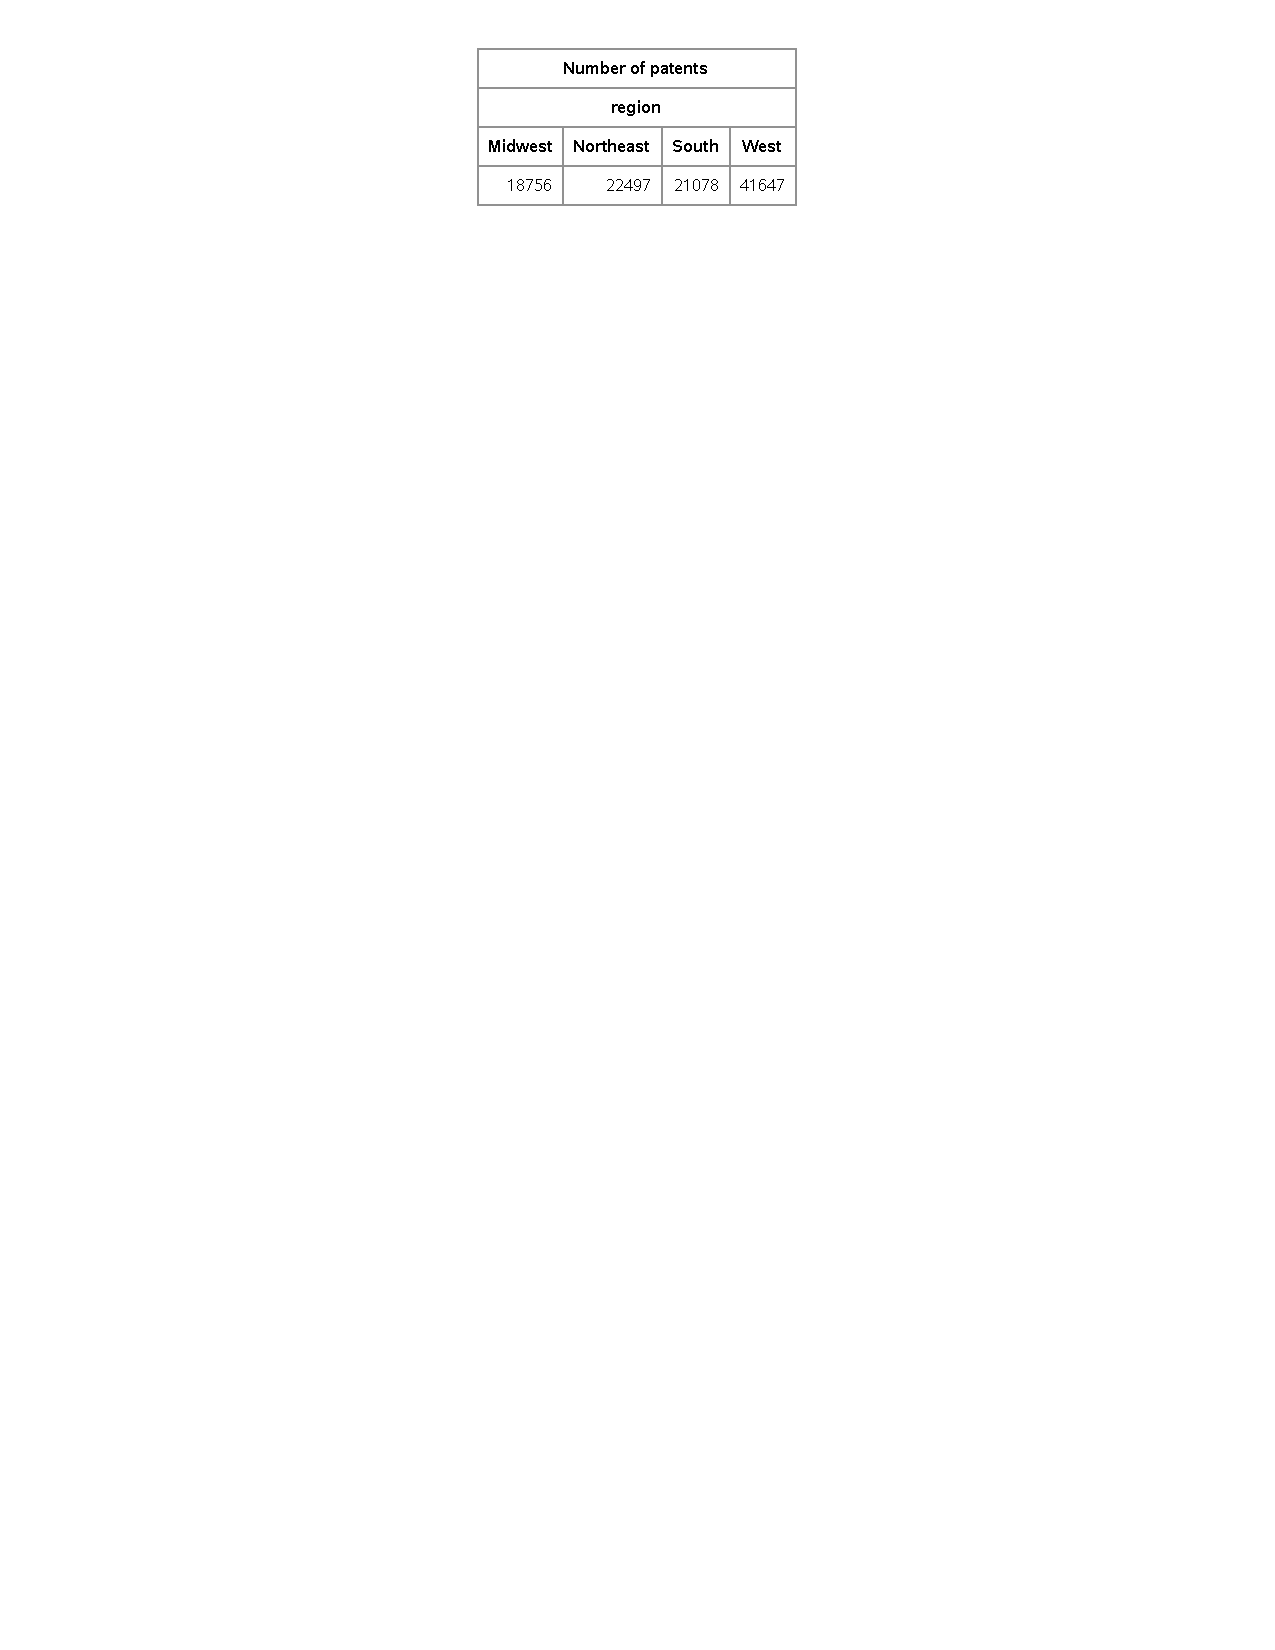
\includegraphics[trim={8cm 24cm 8cm 0.5cm},clip,width=0.5\textwidth]{Lec17Discuss3.pdf}
\end{center}
\bmp{0.50\textwidth}
\begin{code}{.}
PROC REPORT DATA = patents;
   COLUMN Patents \textcolor{OrangeRed}{\fbox{?}} Region;
   DEFINE Region / \textcolor{OrangeRed}{\fbox{?}};
RUN;
\end{code}
\emp
\bmp{0.05\textwidth} \hspace{0.05in} \emp
\bmp{0.45\textwidth}
\begin{clicker}{Fill in the ?:}
\begin{enumerate}
\item \ttt{* } \ttt{ACROSS}
\item \ttt{, } \ttt{ACROSS} %correct
\item \ttt{* } \ttt{GROUP}
\item \ttt{, } \ttt{GROUP}
\end{enumerate}
\end{clicker}
\emp
\end{frame}


%===========================================================================================================================
\section[More]{More}
%===========================================================================================================================
\subsection{}
\begin{frame}
\tableofcontents[currentsection, hideallsubsections]
\end{frame}

%\begin{frame}
%\ft{Breaks}
%Places summary line at the end of the report:
%\vskip5pt
%\fbox{\ttt{rbreak after / summarize;}}
%\vskip20pt
%Places summary line after each \ttt{region}:
%\vskip5pt
%\fbox{\ttt{break after region / summarize;}}
%\vskip20pt
%Breaks can also go \ttt{before}.
%\end{frame}

\begin{frame}[fragile]
\ft{Breaks}
\bmp{1.0\textwidth}
\begin{code}{.}
PROC REPORT DATA = patents SPANROWS;
   COLUMN region division N patents income ;
   DEFINE region / GROUP;
   DEFINE division / GROUP;
   DEFINE patents / ANALYSIS "Patents" F=COMMA10. ;
   DEFINE income / ANALYSIS MEAN "Ave Income" F=DOLLAR10.;
   \textcolor{OrangeRed}{BREAK AFTER region / SUMMARIZE;}
   \textcolor{OrangeRed}{RBREAK AFTER / SUMMARIZE;}
RUN;
\end{code}
\emp
%\blankcolumn
%\bmp{0.35\textwidth}
\vspace{5pt}
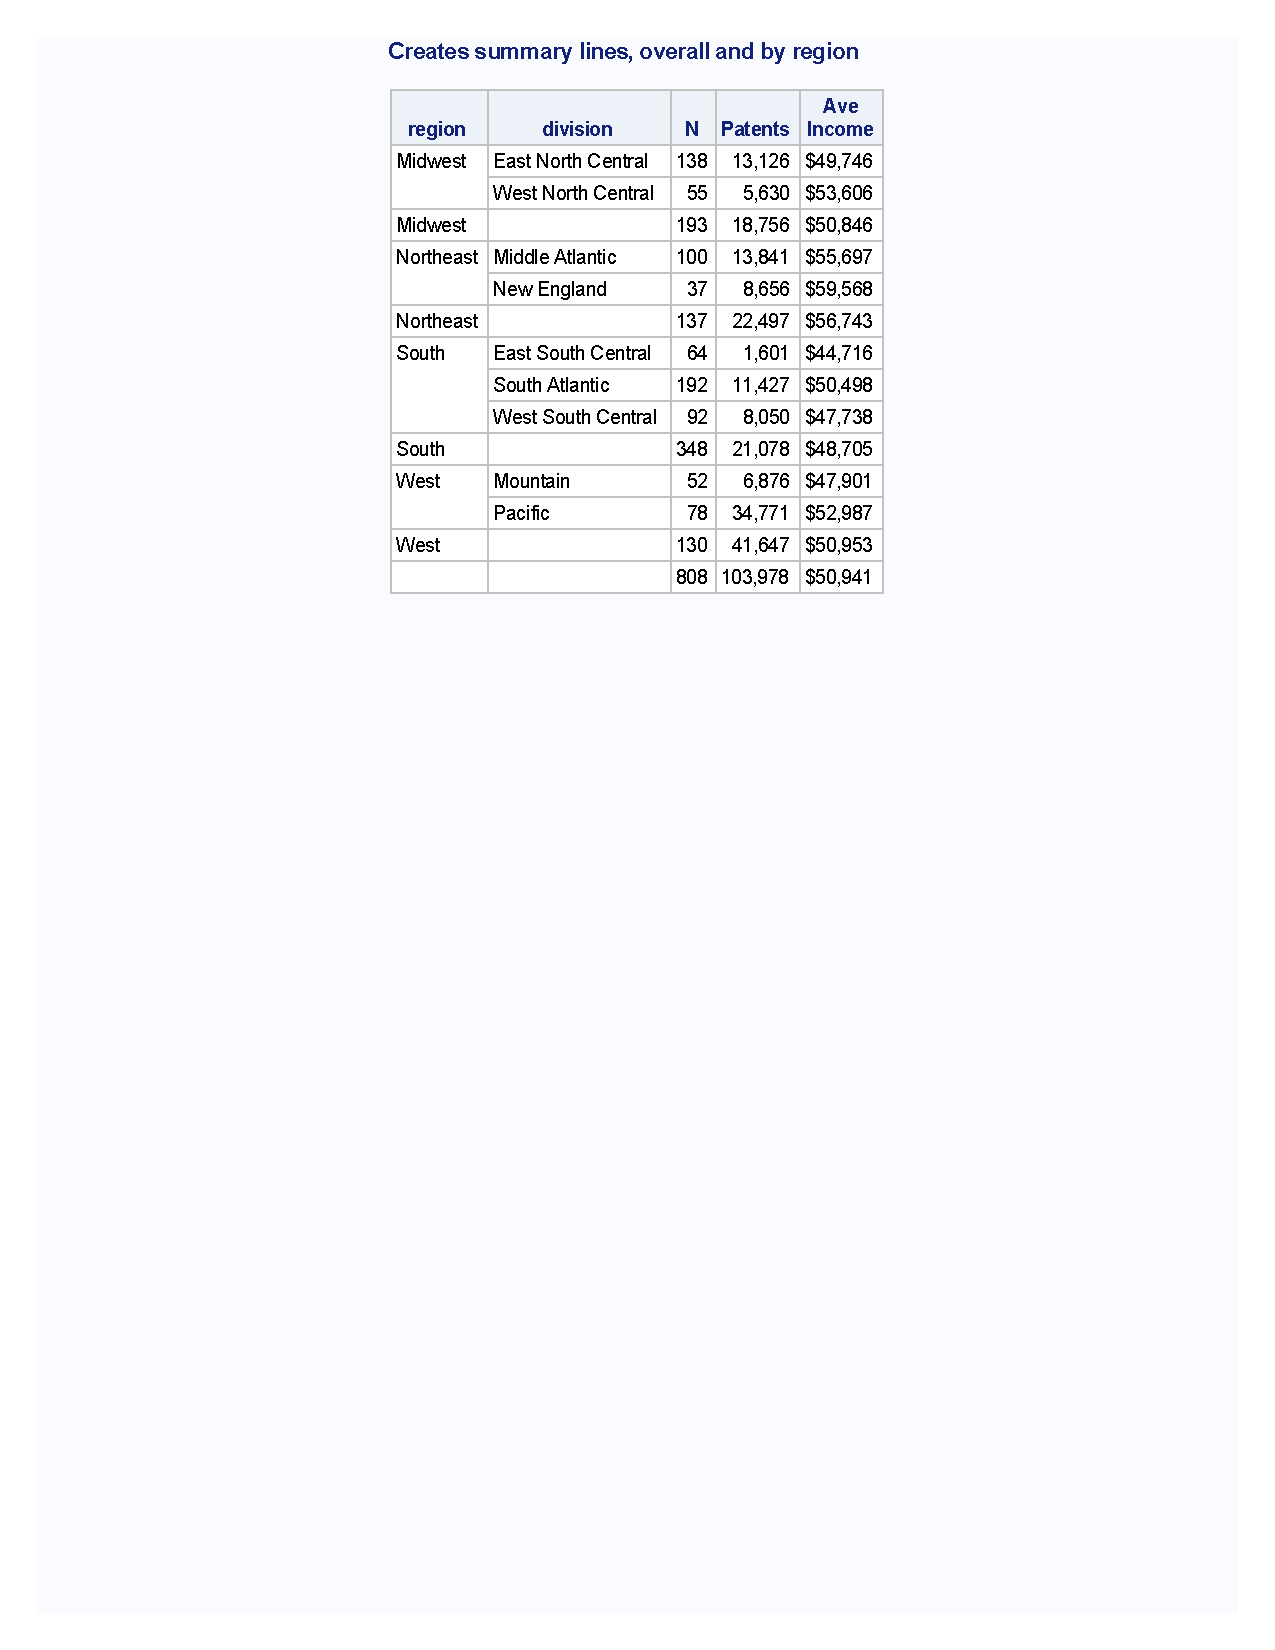
\includegraphics[trim={6cm 17.5cm 6cm 1.5cm},clip,width=0.30\textwidth]{L16_breaks.pdf}\\
%\emp
\end{frame}


\begin{frame}[fragile]
\ft{More things you can do with \ttt{PROC REPORT}}
\bmp{0.65\textwidth}
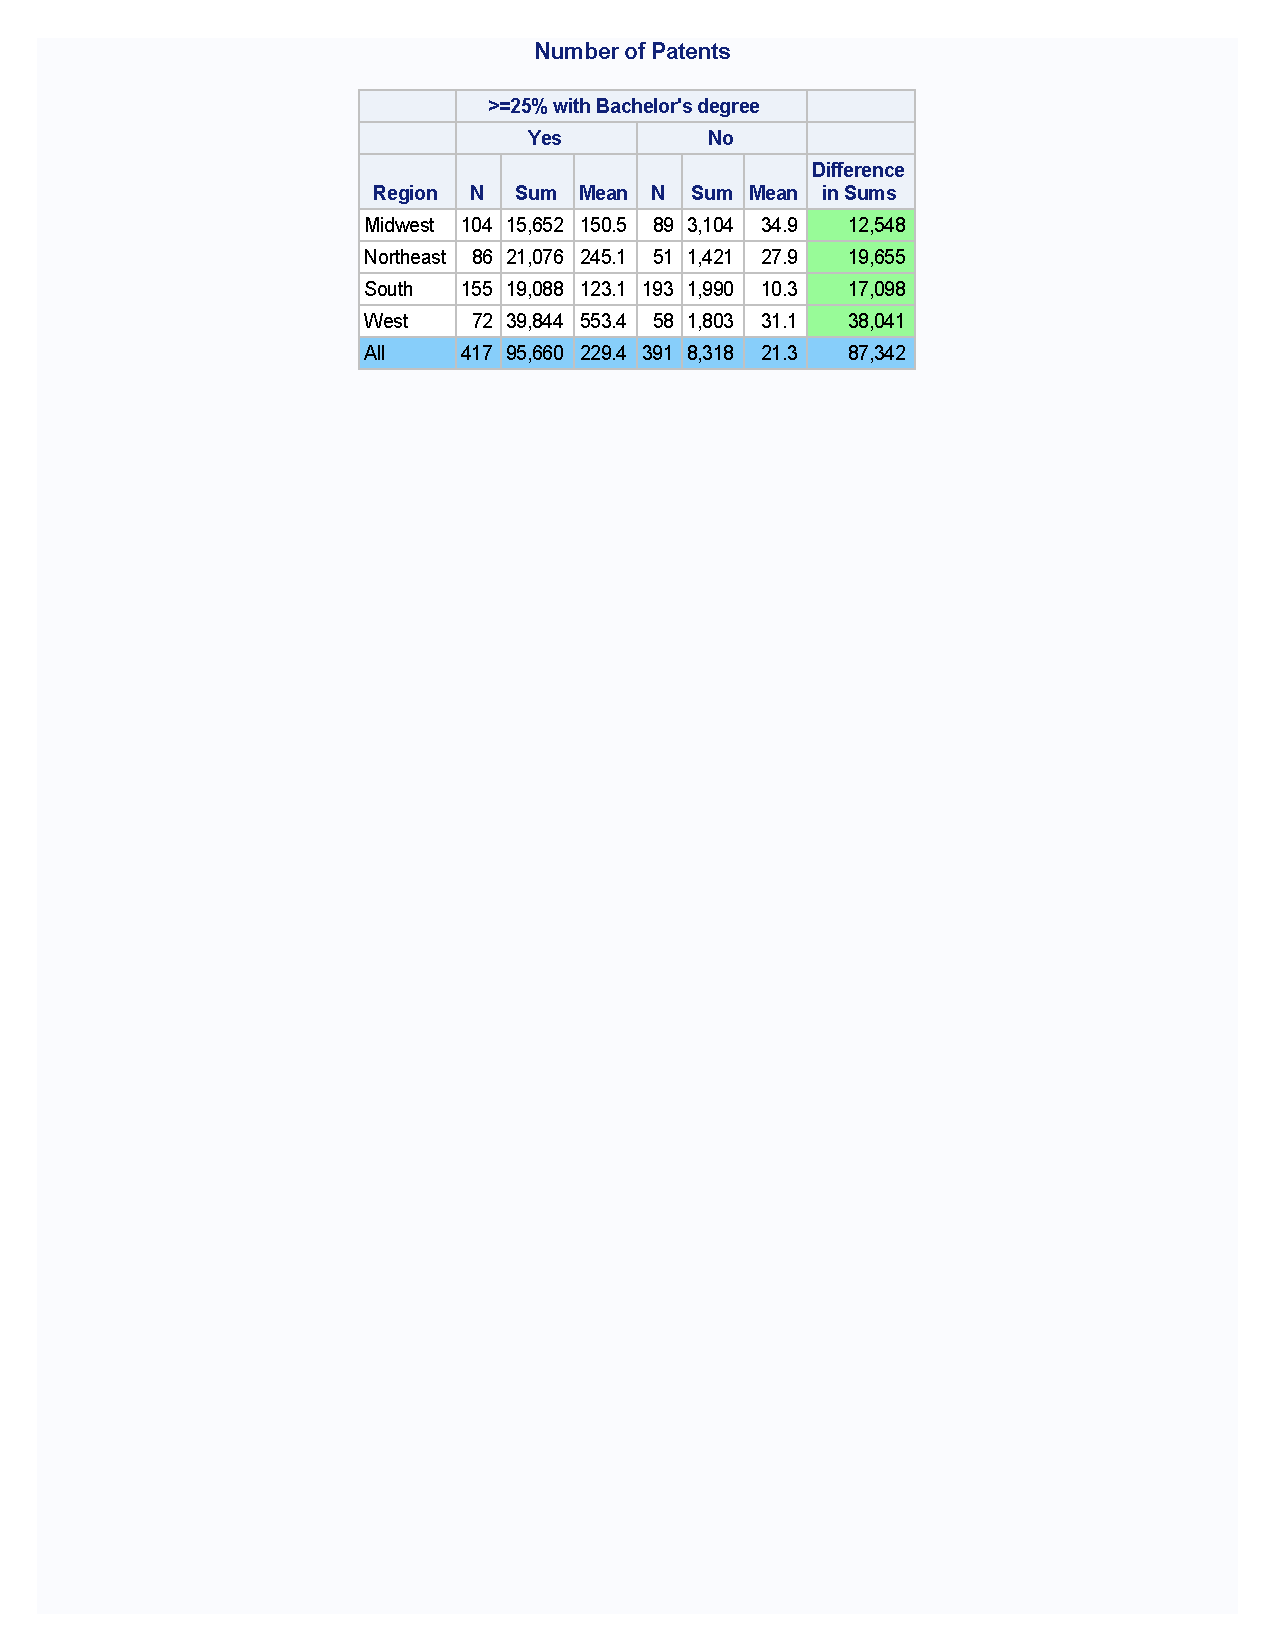
\includegraphics[trim={6cm 21cm 6cm 1cm},clip,width=1.0\textwidth]{L16_more.pdf}
\emp
\blankcolumn
\bmp{0.35\textwidth}
\bi
\item Highlight cells
\item Customize break lines
\item Calculate variables that aren't in the input data set
\ei
\emph{See SAS code corresponding to lecture for full details.}
\emp
\end{frame}

\begin{frame}[fragile]
\ft{Syntax to calculate a new variable}
\bmp{0.6\textwidth}
\begin{code}{.}
PROC REPORT DATA = \emph{mydata};
   COLUMN \emph{var1} \emph{var2} \textcolor{OrangeRed}{\emph{newvar}};
   DEFINE \emph{var1} / analysis;
   DEFINE \emph{var2} / analysis;
   DEFINE \textcolor{OrangeRed}{\emph{newvar}} / COMPUTED ;
   COMPUTE \textcolor{OrangeRed}{\emph{newvar}} ;
       \textcolor{OrangeRed}{\emph{newvar}} = \emph{expression} ;
   ENDCOMP;
RUN;
\end{code}
\emp
\bmp{0.05\textwidth} \hspace{0.05in} \emp
\bmp{0.4\textwidth}
There are many ways to write the \emph{expression}.  One way is to use \fbox{\ttt{\_Cn\_}} where \ttt{n} is the column number.
\emp
\end{frame}

\begin{frame}[fragile]
\ft{PROC REPORT vs PROC TABULATE}
\begin{tabular}{lcc}
\hline
 & \ttt{PROC REPORT} & \ttt{PROC TABULATE} \\
 \hline \hline
 Create summary tables & \gc & \gc \\
 \hline
Create detail tables & \gc & \rx \\
Lines between groups & \gc & \rx \\
Calculate new item & \gc & \rx \\
\hline
Multiple nested variables & \rx & \gc \\
Statistics options & less & more \\
\hline
\end{tabular}
\end{frame}

\end{document} 